\documentclass[12pt]{report}
\usepackage[utf8]{inputenc}

\usepackage{graphicx}
\graphicspath{{images/}}
\usepackage{subcaption}
\usepackage{appendix}
\usepackage[a4paper, width=150mm, top=25mm, bottom=25mm]{geometry}
% \usepackage{fancyhdr}
\usepackage[section]{placeins}

% \pagestyle{fancy}
% \fancyhead[RO, LE]{Thesis Title}



\title{Thesis Title}
\author{Vishal Pandey}
\date{17th May 2020}

\pagenumbering{roman}

\begin{document}


%!TEX root = main.tex
\begin{titlepage}
	\begin{center}
	
		% \vspace*{1cm}
		
		\Large
		\textbf{TRANSFER LEARNING FOR TIME SERIES IMPUTATION IN WIRELESS SENSOR NETWORK}
		
		\vspace{0.5cm}
		\large
		\textit{A dissertation report submitted in partial fullfilment of the requirement for the award of the degree of}
		
		\vspace{1.5cm}
		\textbf{MASTER OF TECHNOLOGY}\\
		\textbf{in}\\
		\textbf{ARTIFICIAL INTELLIGENCE AND ROBOTICS}\\
		
		\vfill
				
		% \vspace{0.8cm}
		
		
\includegraphics[width=0.4\textwidth]{logo}\\

		\vfill
		
		\textbf{SUBMITTED BY:}\\
		\vspace{0.1cm}
		\textbf{VISHAL PANDEY}\\
		\textbf{15/ICS/076}
		
		\vspace{0.5cm}
		\textbf{SUPERVISED BY:}\\
		\vspace{0.1cm}
		\textbf{Dr. VIDUSHI SHARMA}\\
		\textbf{(Assistant Professor)}
		



		\vfill
		\normalsize
		\textbf{SCHOOL OF INFORMATION AND COMMUNICATION TECHNOLOGY} \\
		\textbf{GAUTAM BUDDHA UNIVERSITY} \\
		\textbf{GREATER NOIDA - 201312, UTTAR PRADESH, INDIA} \\
		\textbf{MAY, 2020}
		
	\end{center}
\end{titlepage}

%!TEX root = main.tex
\thispagestyle{plain}
\begin{center}

	\normalsize
	\textbf{SCHOOL OF INFORMATION AND COMMUNIOCATION TECHNOLOGY}\\
	\textbf{GAUTAM BUDDHA UNIVERSITY}\\
	\textbf{GREATER NOIDA - 201312}

	\vspace{0.5cm}

	
\includegraphics[width=0.3\textwidth]{logo}\\
	\Large
	\textbf{Candidate's Declaration}

\end{center}

\normalsize
I here by declare that the work embidied in this dissertation entitled "TRANSFER LEARNING FOR TIME SERIES IMPUTATION IN WIRELESS SENSOR NETWORK" is submitted for the partial fulfillment of the requirements to award the degree of Integrated M.Tech (Artificial Intelligence and Robotics) to School of Information and Communication Technology(ICT), Gautam Buddha Univesity, Freater Noida. It is an authentic record and my own bonafied work has been carried out under the supervision of Dr. Vidushi Sharma, School of ICT. This work is correct to the best of my knowledge and belief and has been undertaken taking care of engineering ethics. It contains no material previously published or written by another person nor material which has been accepted for the award of any other degree or diploma af any university or other institute of higher learning, exceptt where due acknowledgement has been made in the text. Responsibility for any plagiarism related issue stands solely with me.\\

.\\
Name of student: Vishal Pandey\\
Roll No. 15/ICS/076\\
Signature:\\
Date: \\
Place: Greater Noida\\

\addcontentsline{toc}{chapter}{\numberline{}Declaration}
\setcounter{page}{2}

%!TEX root = main.tex
\thispagestyle{plain}
\begin{center}

	\normalsize
	\textbf{SCHOOL OF INFORMATION AND COMMUNIOCATION TECHNOLOGY}\\
	\textbf{GAUTAM BUDDHA UNIVERSITY}\\
	\textbf{GREATER NOIDA - 201312}

	\vspace{0.5cm}

	
\includegraphics[width=0.3\textwidth]{logo}\\
	\Large
	\textbf{Certificate}

\end{center}

\normalsize
This is to certify that work entitled "USING TRANSFER LEARNING FOR TIME SERIES IMPUTATION IN WIRELESS SENSOR NETWORK" by "Vishal Pandey" Roll No. 15/ICS/076 Integrated M.Tech final year with specialisation "ARTIFICIAL INTILLEGENCE AND ROBOTICS" has been carried under my supervision.\\

.\\
\textbf{Dr. Vidushi Sharma}\\
Assistant Professor\\
School Of ICT\\
Gautam Buddha University\\
Greater Noida, 201312\\
(Uttar Pradesh India)

\addcontentsline{toc}{chapter}{\numberline{}Certificate}
\setcounter{page}{3}

%!TEX root = ./main.tex
\begin{center}
	\Large
	\textbf{ACKNOWLEDGMENT}
\end{center}
Throughout my dissertation, I have been very fortunate to get help and support from many people. I feel immense pleasure in expressing my profound gratitude to my supervisor, Dr. Vidushi Sharma, SOICT, for her guidance, useful suggestion, and for permitting me to carry out this work, which helped me complete the work on time. She inspired me greatly to work on this dissertation. Her willingness to motivate me contributed tremendously to work. I would like to thank her for showing me a few examples related to the topic in my dissertation.

I would like to acknowledge Dr. Anurag Singh Baghel, for his encouragement that boosted my morale and confidence, I would like to express my gratitude and heartfelt thanks to Dr. Neeta Shing, for her excellent supervision and support in his research.

Besides, I  would like to thank the authority of the School of Information and Communication Technology (ICT), Gautam Buddha University, for providing a good environment and facilities that helped me complete this dissertation.

I Would like to express my heartfelt thanks to my beloved parents for their blessings and whiches for the successful completion of this work. Last but not least, Almighty God has been the invisible divine force behind my accomplishments.
\\
\\
Vishal Pandey
\\
15/ICS/076\\
\addcontentsline{toc}{chapter}{\numberline{}Acknowledgement}
\setcounter{page}{4}

%!TEX root = main.tex
\thispagestyle{plain}

	\begin{center}
		\Large
		\textbf{ABSTRACT}
	\end{center}
	IoT is a field that combines the capability of two domains: computer science and electronics. IoT devices are basically sensor nodes (usually wireless) connected to each other and to the central control system through the internet. Various applications IoT is in healthcare, weather monitoring, remote control, collecting data from sensors. Missing data in the wireless sensor network is inevitable and is a major field of study since the start of IoT and WSN. IoT operates in technologies which are lossy networks. There may be many reasons for the loss of data while communication one of the reason may be confession the other reason being a loss in tunning of duty cycles of sender and receiver and other environmental condition in which they operate. Recovering the lost data is important in mission-critical applications such as health care, defense etc. In IoT networks to overcome these issues and regenerate the data machine learning techniques can prove to be beneficial since the IoT networks have constraint devices so robust and complex techniques do not fit in their communication model.   \\
\addcontentsline{toc}{chapter}{\numberline{}Abstract}
\setcounter{page}{5}

\listoffigures
\addcontentsline{toc}{chapter}{\numberline{}List of figures}
\setcounter{page}{6}

\listoftables
\addcontentsline{toc}{chapter}{\numberline{}List of tables}
\setcounter{page}{7}

%!TEX root = ./main.tex
\thispagestyle{plain}
\begin{titlepage}
\huge
\textbf{List of abbreviation}\\

\normalsize
\noindent
\textbf{SSIM} \hfill Sequence to Sequence Imputation Model \\
\textbf{LSTM} \hfill Long Short Term Memory \\
\textbf{MSE} \hfill Mean Squared Error \\
\textbf{WSN} \hfill Wireless Sensor Network \\
\textbf{GPS} \hfill Global Positioning System \\
\textbf{LED} \hfill Light Emiting Diode \\
\textbf{RF} \hfill Radio Frequency \\
\textbf{AI} \hfill Artificial Intelligence \\
\textbf{DL} \hfill Deep Learning \\
\textbf{RNN} \hfill Recurrent Neural Network\\
\textbf{TL} \hfill Transfer Learning\\
\textbf{EMG} \hfill Electromyographic\\
\textbf{EEG} \hfill Electroencephalographic\\
\textbf{ARIMA} \hfill Autoregressive integrated moving average\\
\textbf{VLSW} \hfill Variable Length Sliding Window\\
\textbf{MQTT} \hfill Message Queueing Telementary Transport\\
\textbf{COAP} \hfill Constrained Application Protocol\\
\textbf{PM2.5} \hfill Particulate Matter diameter less than 2.5 micrometer \\
\textbf{DNN} \hfill Deep Neural Network\\

\end{titlepage}
\addcontentsline{toc}{chapter}{\numberline{}List of abbreviation}
\setcounter{page}{8}

\tableofcontents
\newpage
\pagenumbering{arabic}
\chapter{Introduction}
%!TEX root = ../main.tex
\section{Overview}
Wireless sensor network is a type of network which is wireless used for sensing purpose. It is a collections of various amount of sensors available in a network which are connected wirelessly. The main component of the wireless sensor network are sensor nodes. Sensor nodes play an important role in the working of this entire network system. Sensor nodes act as a powerful component for doing various activities like communication, sensing and data interpretation. The wireless network system is a remarkable tool in technology which ease the computational work to a great extend. The use of the wireless sensor network technology helps the work of data interpretation so fast and accurate. The errors causes by human intervention in the process at communication and networking can be completely sabotaged by the use of this technology. Using the concept of wireless communication, network system and various sensor theories makes this entire system work efficiently and with remarkable accuracy.

\section{Wireless Sensor Network}

In recent time their is more ease with  communication, and computation because of advances in processor, memory, and radio technology enable small and cheap nodes capable of sensing,. Distributing sensing of environmental having networks of such nodes can coordinate to perform  phenomena. With a wide range of applications in areas such as traffic monitoring\cite{1}, medical care\cite{2}, in hospitable terrain, robotic exploration\cite{3}, and agriculture surveillance\cite{4}. The advent of efficient wireless communications and advancement in electronics has enabled the development of low-power, low-cost, and multifunctional wireless sensor nodes that are characterized by miniaturization and integration.

The network uses location information to reduce redundant transmissions, thereby saving energy. The sensor network is divided into virtual grids and each sensor node associates itself with a virtual grid based on its location. Sensor nodes within a virtual grid are classified as either gateway nodes or internal nodes. While gateway nodes are responsible for forwarding the data across virtual grids, internal nodes forward the data within a virtual grid. In order to make communications both reliable and energetic efficient Deep learning approch is used.

Wireless Sensor Networks (WSNs) can be defined as a self-configured and infrastructure less wireless networks to monitor physical or environmental conditions, such as temperature, sound, vibration, pressure, motion or pollutants and to cooperatively pass their data through the network to a main location or sink where the data can be observed and analysed. A sink or base station acts like an interface between users and the network. One can retrieve required information from the network by injecting queries and gathering results from the sink. Typically a wireless sensor network contains hundreds of thousands of sensor nodes. The sensor nodes can communicate among themselves using radio signals. A wireless sensor node is equipped with sensing and computing devices, radio transceivers and power components. The individual nodes in a wireless sensor network (WSN) are inherently resource constrained: they have limited processing speed, storage capacity, and communication bandwidth. After the sensor nodes are deployed, they are responsible for self-organizing an appropriate network infrastructure often with multi-hop communication with them. Then the onboard sensors start collecting information of interest. Wireless sensor devices also respond to queries sent from a “control site” to perform specific instructions or provide sensing samples. The working mode of the sensor nodes may be either continuous or event driven. Global Positioning System (GPS) and local positioning algorithms can be used to obtain location and positioning information\cite{5}. Wireless sensor devices can be equipped with actuators to “act” upon certain conditions.


Wireless sensor networks (WSNs) enable new applications and require non-conventional paradigms for protocol design due to several constraints. Owing to the requirement for low device complexity together with low energy consumption (i.e. long network lifetime), a proper balance between communication and signal or data processing capabilities must be found. This motivates a huge effort in research activities, standardization process, and industrial investments on this field.


Wireless sensor networks are used in environmental trackings, such as forest detection\cite{6}, animal tracking\cite{7}, flood detection\cite{8}, forecasting and weather prediction\cite{9}, and also in commercial applications like seismic activity prediction and monitoring.Irrespective of the application, Wireless Sensor Networks in general can be classified into the following categories\cite{10}.

\begin{itemize}
\item Static and Mobile WSN.
\item Deterministic and Nondeterministic WSN.
\item Single Base Station and Multi Base Station WSN.
\item Static Base Station and Mobile Base Station WSN.
\item Single-hop and Multi-hop WSN.
\end{itemize}


The components of WSN system are sensor node, rely node, actor node, cluster head, gateway and base station. a. Sensor node: Capable of executing data processing, data gathering and communicating with additional associated nodes in the network.


A sensor node, also known as a node in a sensor network that is capable of performing some processing, gathering sensory information and communicating with other connected nodes in the network. A mote is a node but a node is not always a mote.


A Wireless sensor network can be defined as a network of devices that can communicate the information gathered from a monitored field through wireless links\cite{11}. The data is forwarded through multiple nodes, and with a gateway, the data is connected to other networks like wireless Ethernet.


A Wireless sensor network can be defined as a network of devices that can communicate the information gathered from a monitored field through wireless links. The data is forwarded through multiple nodes, and with a gateway, the data is connected to other networks like wireless Ethernet.


There are various features one of them is linearity which represents the relationship between input variations and output variations.Second is frequency response: The frequency response is the range i to the input remains relatively high.Third is reliability.Fourth is accuracy.Fifth is repeatability and other features are size, weight and volume.


A sensor consists of three main components in which the sensing section contains the sensor itself which is based on a particular technology and the processing circuitry converts the physical variable into an electrical variable in which the signal output contains the electronics connected to a control system.The base stations are one or more components of the WSN with much more computational, energy and communication resources. They act as a gateway between sensor nodes and the end user as they typically forward data from the WSN on to a server.


Sensor nodes are used for constant sensing, event ID, event detection \& local control of actuators. They convert physical or monitored signals like temperature, motion or light intensity to electrical signals. They are composed of a transistor, a resistor and an LED. Connect the resistor and LED in series from the positive supply to the collector of the transistor. Connect the emitter of the transistor to the negative terminal of the supply. Create two wires with exposed ends.


Most sensors use wireless RF signals, a hardwired connection or WIFI connectivity. These devices communicate primarily using RF signals. The electrical signals are transmitted to reciever either by wired communication or wireless communication.


Through sensors there is an imporvement in many fields like diagnostics in medical applications; improved performance of energy sources like fuel cells and batteries and solar power; improved health and safety and security for people; sensors for exploring space and the known university; and improved environmental monitoring.


They are classified into three categories: passive, omnidirectional sensors; passive, narrow-beam sensors; and active sensors. Passive sensors sense the data without actually manipulating the environment by active probing. They are self powered; that is, energy is needed only to amplify their analog signal.The most frequently used different types of sensors are classified based on the quantities such as Electric current or Potential or Magnetic or Radio sensors, Humidity sensor, Fluid velocity or Flow sensors, Pressure sensors, Thermal or Heat or Temperature sensors, Proximity sensors, Optical sensors, Position sensors.These sensors connect  to a microcontroller (uC), then connect uC to the PC through a USB or RS-232 or Bluetooth.


Challenges in such WSN include high bandwidth demand, high energy consumption, quality of service (QoS) provisioning, data processing and compressing techniques, and cross-layer design. physical environment\cite{12}. Mobile nodes have the ability to sense, compute, and communicate like static nodes.


Wireless network is basically based on sensory nodes. These sensory nodes act as the information carrier in the whole network system . these sensory nodes are scattered in the field called sensory field from where the network system does the work of data collection. The sensory field is the place from where the sensory nodes collect the data required for the designed system. The data after collection is transmitted and requires actions are taken on it and final processing takes place over the transmitted data. The data after the processing from the sensory field is directed toward the sink which is called as ‘gateway’. This is how the compelet wireless sensorey network is designed in this arcitectural pattern. This architecture is uses used in building the model to get the required task executed.


\section{Deep Learning and Data Science}

Data Science approach is used to solve the problems related to data. It tells automatically which features to use for calculation. A subset of it is AI. A subset of it is Deep Learning where the same function is applied again and again. Figure \ref{fig:deeplearning} Describes the classificiation of deep learning.


\begin{figure}[ht]
	\centering
	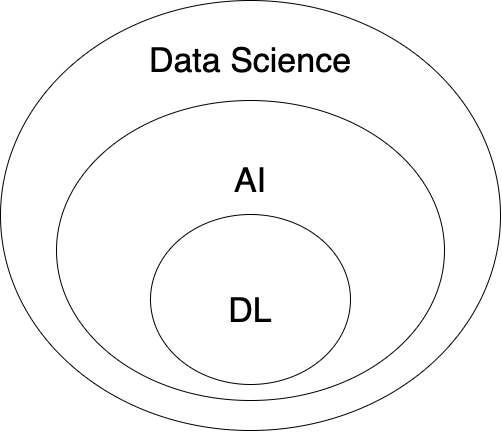
\includegraphics[width=0.8\textwidth]{images/deep-learning}
	\caption{Deep Learning Hirarchy}
	\label{fig:deeplearning}
\end{figure}


Walter Pitts and Warren McCulloch created a computer model based on the neural networks of the human brain\cite{13}. They used a combination of algorithms and mathematics they called “threshold logic” to match the thought process.

Deep learning is a subset of machine learning where artificial neural networks, algorithms inspired by the human brain, learn from large amounts of data\cite{14}. Deep learning allows machines to solve complex problems even when using a data set that is very diverse, unstructured and inter-connected. If there are more than three layers (including input and output) it will qualify as “deep” learning.

Deep learning systems represent the first time computers can understand images at a useful level and reasonable cost. The majority of jobs involve some form of visual perception. ie detection and classification of visual information.

Deep Learning uses a Neural Network to imitate animal intelligence. There are three types of layers of neurons in a neural network: the Input Layer, the Hidden Layer(s), and the Output Layer. Connections between neurons are associated with a weight, dictating the importance of the input value.

Deep learning is a machine learning technique that teaches computers to do what comes naturally to humans. In deep learning, a computer model learns to perform classification tasks directly from images, text, or sound.

Deep learning networks can be successfully applied to big data for knowledge discovery, knowledge application, and knowledge-based prediction. In other words, deep learning can be a powerful engine for producing actionable results

A Deep feature is a consistent response of a node or layer within a hierarchical model to an input that gives a response that's relevant to the model's final output. One feature is considered “deeper” than another depending on how early in the decision tree or other framework the response is activated.

Deep learning is an increasingly popular subset of machine learning. Deep learning models are built using neural networks. A neural network takes in inputs, which are then processed in hidden layers using weights that are adjusted during training. Then the model spits out a prediction. The number of layers of neurons stacked is greater than what's done in Machine Learning, so you now have deep neural networks. Deep Learning is a subset of Machine Learning. Deep learning consists of neural networks with many hidden layers which makes the layers deep. Deep learning then can be defined as neural networks with a large number of parameters.

The layers in one of four fundamental network architectures\cite{15}:
\begin{itemize}

\item Unsupervised Pre-trained Networks.
\item Convolutional Neural Networks.
\item Recurrent Neural Networks.
\item Recursive Neural Networks.
\end{itemize}
Deep learning architectures such as deep neural networks, deep belief networks, recurrent neural networks and convolutional neural networks have been applied to fields including computer vision, speech recognition, natural language processing, audio recognition, social network filtering, machine translation. Its applications are used in industries from automated driving to medical devices. Automated Driving: Automotive researchers are using deep learning to automatically detect objects such as stop signs and traffic lights. In addition, deep learning is used to detect pedestrians, which helps decrease accidents. he 'deep' in deep learning simply refers to having multiple 'hidden' layers; that is layers that aren't the input, or the final output, but somewhere in between.

One of the Deep learning algorithm CNN is suitable for spatial data such as images\cite{16}. RNN is suitable for temporal data, also called sequential data\cite{17}. CNN is considered to be more powerful than RNN. They unlike feed-forward neural networks - can use their internal memory to process arbitrary sequences of inputs.

More layers can be better but also harder to train. As adding a second layer only improves the accuracy by approx 0.2\% (0.9807 vs. 0.9819) after 10 epochs.

Long short-term memory (LSTM) is an artificial recurrent neural network (RNN) architecture used in the field of deep learning\cite{18}. LSTM networks are well-suited to classifying, processing and making predictions based on time series data since there can be lags of unknown duration between important events in a time series.

Human mankind always wanted to have the machines which would have the ability to do the reasoning aspect by it itself. Building such a intellectual machine which could do all reasoning work by itself was a big challenge. Having a machine which could function like a human brain and have the capacity to do the logical operations all by itself was huge challenge. A machine which could actually behave like a human brain. Well, that desire of human mankind to have such a computing machine lead to emergence of the concept of AI i.e artificial intelligence. AI is a concept which acted as a great tool to give a huge strength to the computing machines these days. AI has a capacity to work exactly like how human neural system work. Well, the alogrithum used to design any AI concept was inspired by human neural system.

\begin{figure}[ht]
	\centering
	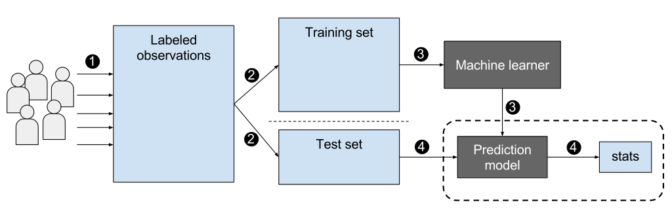
\includegraphics[width=0.8\textwidth]{images/supervised-machine-learning.png}
	\caption{Supervised Machine Learning}
	\label{fig:supervised-machine-learning}
\end{figure}


As the research progressed in the field of AI which lead to have remarkably improved piece of technology , the concept of machine learning came into existence alongside with all of this. Machine learning is an important part of AI.machine learning is a concept where the machine has the capacity to learn by itself from the given set of data in a particular manner.

% \begin{figure}[ht]
% 	\centering
% 	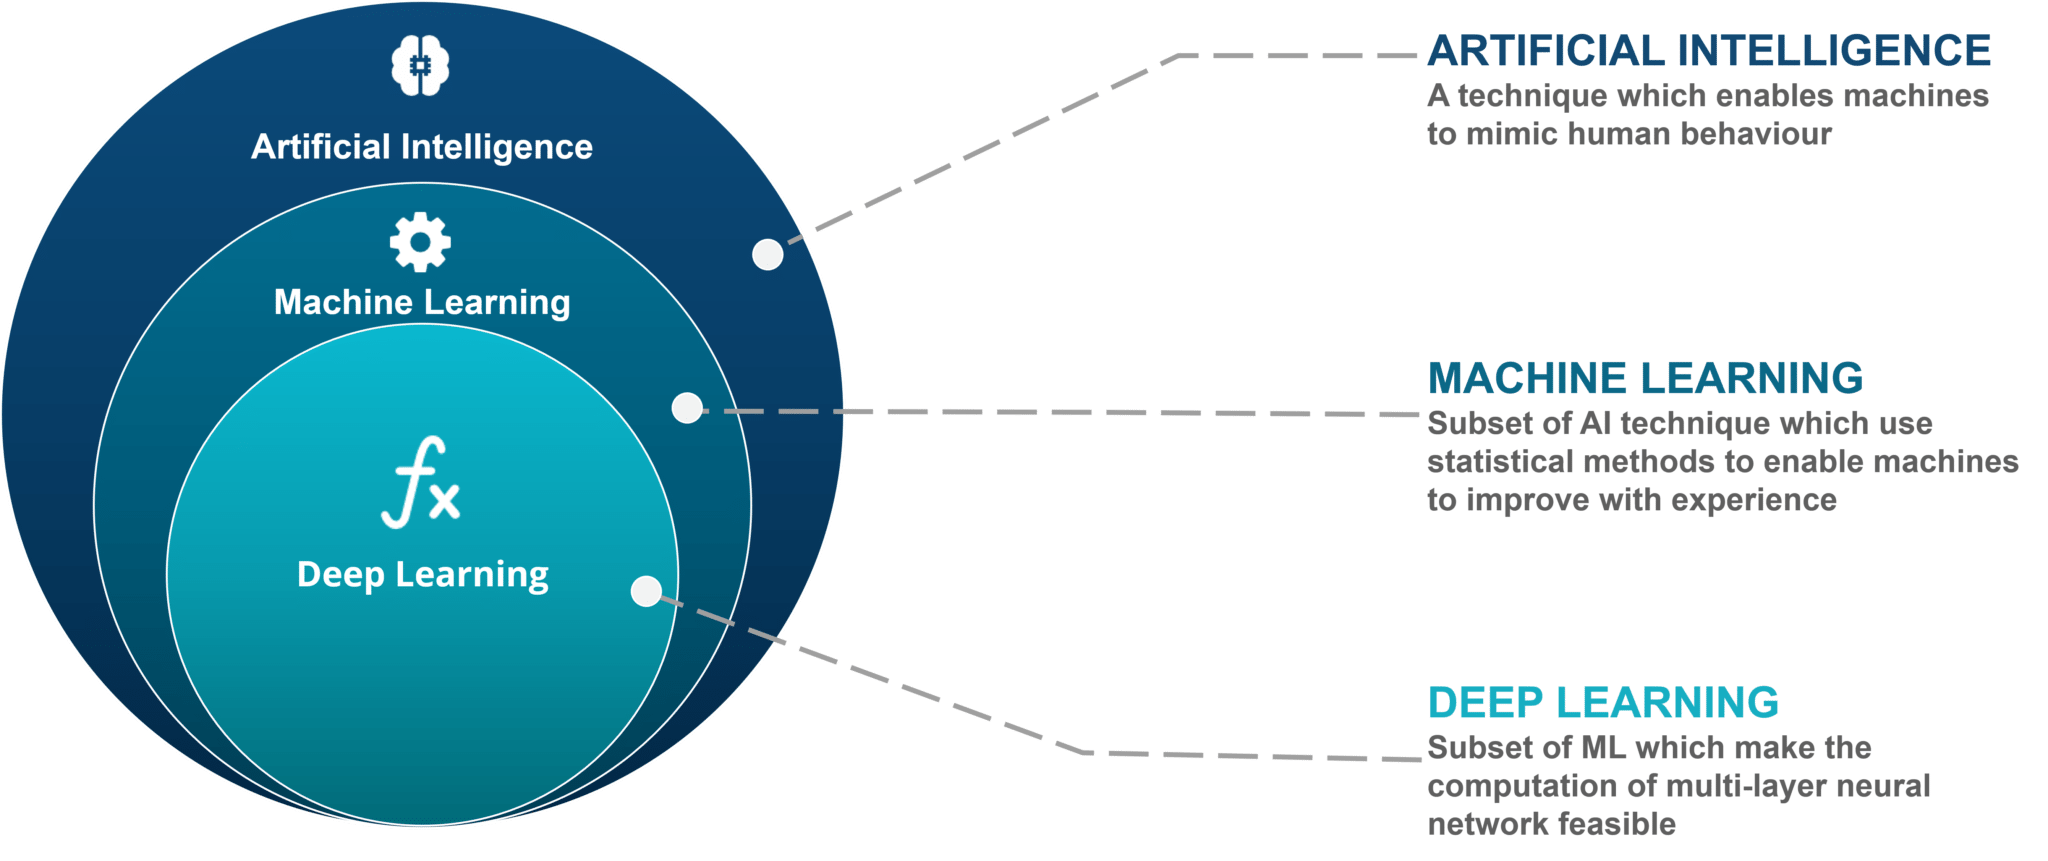
\includegraphics[width=0.8\textwidth]{images/classification-of-ai.png}
% 	\caption{Classification of AI}
% 	\label{fig:classification-of-ai}
% \end{figure}

Earlier the information stored in the system and how the system used to work was based on hard core computational language. The language was more in the numeric form which not giving the freedome of any other sort of interpretation. The language used for these machinery was more scientific. To have a reasoning capability in the machine, there was a huge need of thee development of some different sort of language system. Due to this need, the concept of AI came into existence.

AI gave the computers the reasoning ability and analyise the data using thise reasoning logics.

But later feeding the data everytime to the syste to check the result became a proble. So as to solve such problem, people needed something which could actually self learn the data around the world. So as to accomplish that task, the concept of machine learning came ino existence. Where the concept of machine learning opened the gateway for the machine to self identify and learn from the data available to  them by them selves and act accurately over it.

\begin{figure}[ht]
	\centering
	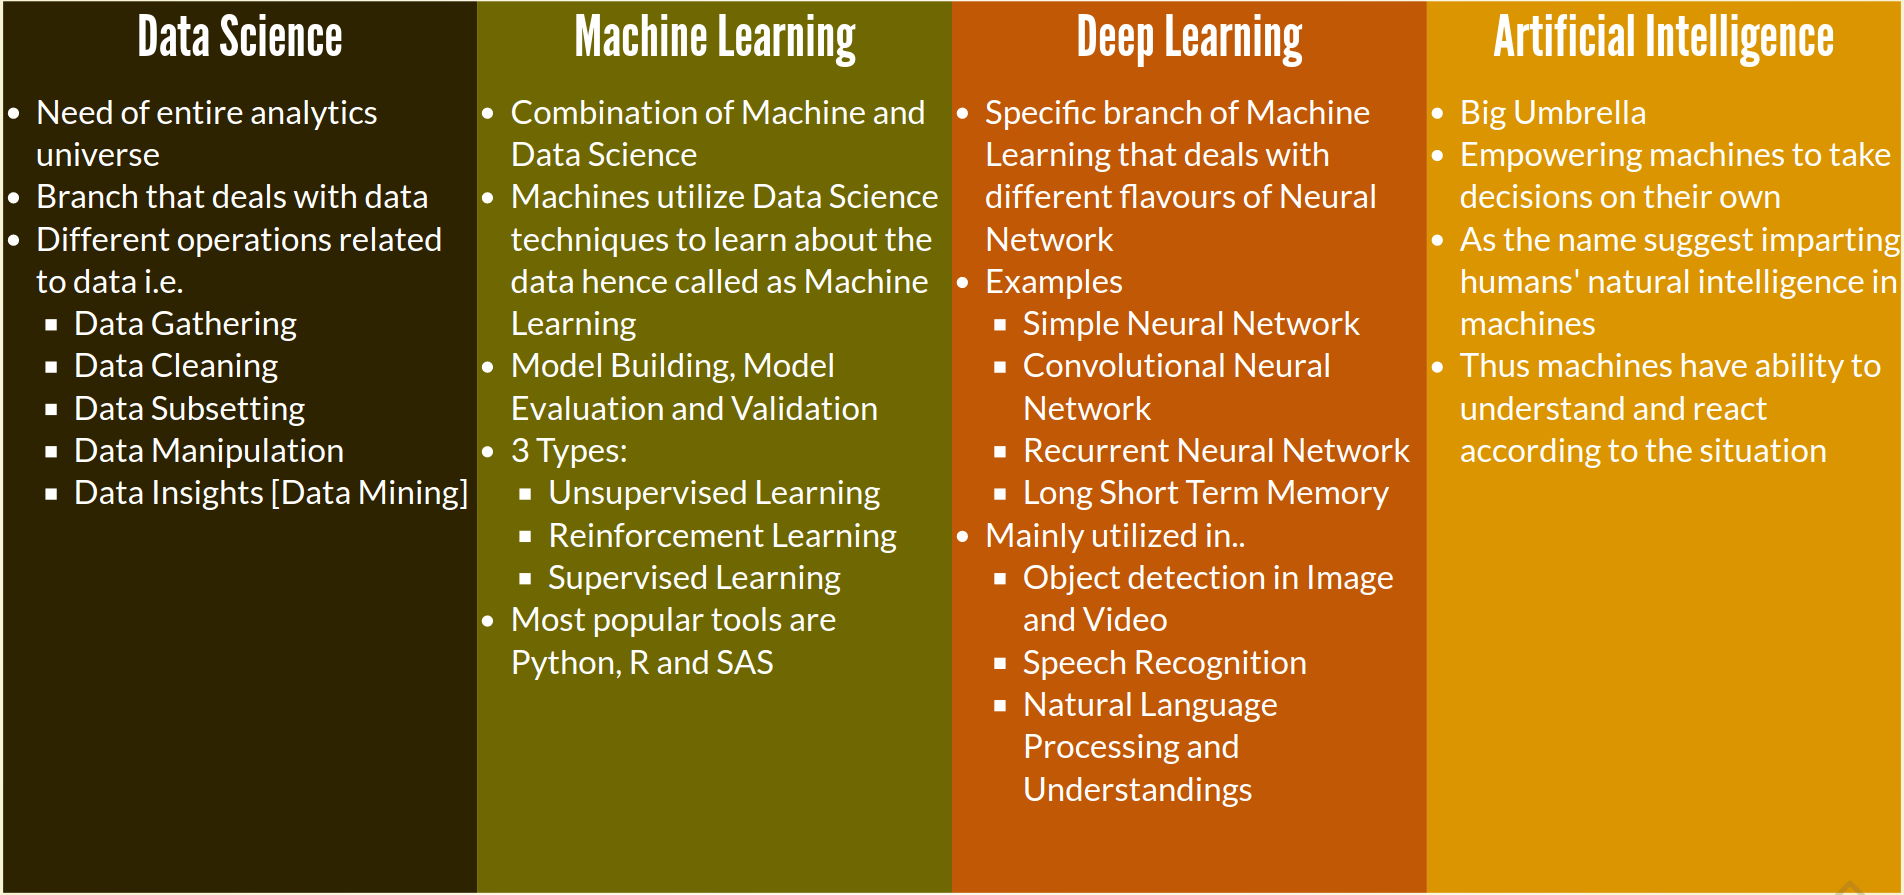
\includegraphics[width=0.8\textwidth]{images/ai.png}
	\caption{Difference between Data Science, ML, DL and, AI }
	\label{fig:ai}
\end{figure}


After this, to solve more complexed problem using AI and using machine learning,  we need more sophisticated tools. From where exactly the concept tof deep learning came into existence. Deep learning is the part of machine learning you can say the eep learning is the subset of the machine learning.

% \begin{figure}[ht]
% 	\centering
% 	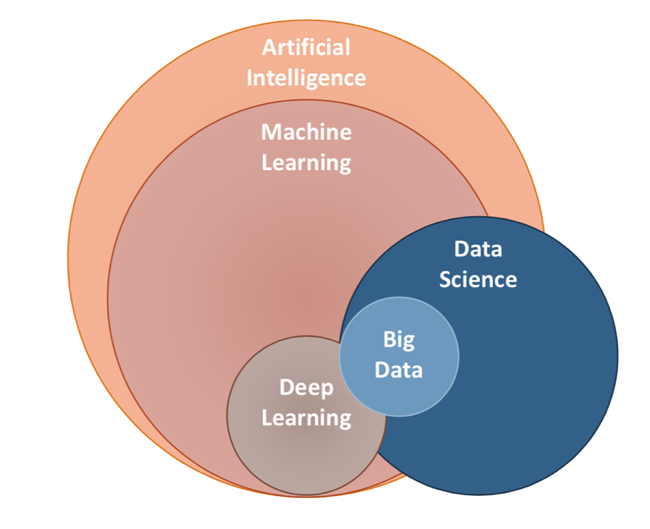
\includegraphics[width=0.8\textwidth]{images/venn-diagram.png}
% 	\caption{Venn Diagram}
% 	\label{fig:venn}
% \end{figure}

Deep learning is majorly used to interpret the data and come up with the conclusions where there is huge lack of segregated data. Where the data available to us is not in a presentable format and completely unorganized, there deep learning act a strong tool to do our analysis over those type of data and retrieve something valuable out of it



\section{Transfer Learning}

Transfer learning (TL) is a research problem in machine learning (ML) that focuses on storing knowledge gained while solving one problem and applying it to a different but related problem\cite{19}. For example, knowledge gained while learning to recognize cats could apply when trying to recognize tigers. This area of research bears some relation to the long history of psychological literature on transfer of learning but from the practical standpoint, reusing or transferring information from previously learned tasks for the learning of new tasks has the potential to significantly improve the sample efficiency of a reinforcement learning agent.

Algorithms are available for transfer learning in Markov logic networks and Bayesian networks. Transfer learning has also been applied to cancer subtype discovery, general game playing, text classification, digit recognition and spam filtering.

In 2020 it was discovered that, due to their similar physical natures, transfer learning is possible between Electromyographic (EMG) signals from the muscles when classifying the behaviours of Electroencephalographic (EEG) brainwaves from the gesture recognition domain to the mental state recognition domain\cite{20}. It was also noted that this relationship worked vice-versa, showing that EEG can likewise be used to classify EMG in addition. The experiments noted that the accuracy of neural networks and convolutional neural networks were improved through transfer learning both at the first epoch and at the asymptote.So algorithms are improved by exposure to another domain.

The main features are: What transfer learning is and how to use it. Common examples of transfer learning in deep learning.When to use transfer learning on your own predictive modelling problems.

Transfer learning is related to problems such as multi-task learning and concept drift and is not exclusively an area of study for deep learning. The transfer learning is popular in deep learning given the enormous resources required to train deep learning models or the large and challenging datasets on which deep learning models are trained. Transfer learning is an optimization, a shortcut to saving time or getting better performance. It is not obvious that there will be a benefit to using transfer learning in the domain until after the model has been developed and evaluated. These features  are required for Transfer learning:

Higher start. The initial skill (before refining the model) on the source model is higher than it otherwise would be.
Higher slope. The rate of improvement of skill during the training of the source model is steeper than it otherwise would be.
Higher asymptote. The converged skill of the trained model is better than it otherwise would be.

\textbf{Two models of Transfer Learning}
\begin{itemize}
	\item Develop a Model Approach
	\item Pre-trained Model Approach
\end{itemize}

\textbf{Develop a Model Approach}

\begin{itemize}
\item Select Source Task. You must select a related predictive modelling problem with an abundance of data where there is some relationship in the input data, output data, and/or concepts learned during the mapping from input to output data.
\item Develop Source Model. Next, you must develop a skilful model for this first task. The model must be better than a naive model to ensure that some feature learning has been performed.
\item Reuse Model. The model fit on the source task can then be used as the starting point for a model on the second task of interest. This may involve using all or parts of the model, depending on the modelling technique used.
\item Tune Model. Optionally, the model may need to be adapted or refined on the input-output pair data available for the task of interest.
\end{itemize}

\textbf{Pre-trained Model Approach}
\begin{itemize}
\item \textbf{Select the Source Model.} A pre-trained source model is chosen from available models. Many research institutions release models on large and challenging datasets that may be included in the pool of candidate models from which to choose from.
\item \textbf{Reuse Model.} The model pre-trained model can then be used as the starting point for a model on the second task of interest. This may involve using all or parts of the model, depending on the modelling technique used.
\item \textbf{Tune Model.} Optionally, the model may need to be adapted or refined on the input-output pair data available for the task of interest.
\end{itemize}



Transfer learning is a different type of machine learning method.
As the concept of machine learning is really important to have good AI based programme
and to have good analytical software. As explained in the starting section about the
emergence of machine learning. Elaborating the importance of the machine learning here.

It is very important to understand the kind of technique we are using for the machine
learning process. As the technique we use for the machine learning process plays a very big
part at how quality results we will receive and how fast the execution of the work will take
place.

So there are various type of machine learning techniques in the market.

Where
1. Supervised learning – in this learning the machine learns by flashing the certain set
of information infront of it. It is like learning like a small kid where the kid learns by
having flash cards.

Some common application of supervised learning are as follows :-

Advertisement clickablity
Identification of spam
Facial recoginition




Unsupervised learning –in this sort of learning the machine is feed with unorganised
data. After feeding the system with the unorganized , the system is allowed to
identify the difference among them by itself.

Some common application of unsupervised learning are as follows :-

  Recommendation system
  Buying behaviour
  Common issue rectifier

Reinforcement learning- In this type of learning the machine learn by iterating the
given data again and again. The machine learning by through same type of data
various times and becoming more accurate about it.

Some common application of reinforcment learning are as follows :-

  Video games
  Industrial management
  Management of resources


Here we will talk about following things about transfer learning
	What is exactly transfer learning
	Real time application of transfer learning
	Productivity impact by using transfer learning.

\section{Challenges and Problem Identification}

Limitations in applying the prediction model in the production environment.
\\

1. Sensor nodes are resource constraint so the prediction model cannot be deployed on sensor nodes.

2. Cluster head can have more resources in comparison to the individual nodes but the machine learning model also cannot be applied there because a cluster head needs to process data collected from a number of different sensor nodes, which intern leave no option to deploy on the cluster head.

3. Machine learning algorithm needs heavy computing generally GPUs are used for the training of the machine learning models, and to be applied in the production environment you have to continue training and updating the model to better adapt for the upcoming missing values, so remote devices are not the choice for the deployment.

4. For training a supervised deep-learning algorithm we need a huge amount of labeled data, which is rare in the IoT and WSN environment.


\section{Motivation}

Cloud computing is a branch of computer science where a network of computers connected to the internet (called cloud) and available for use as per demand.


As there is no limitation in the computing capacity and resources in the cloud and IoT devices are connected to the internet the IoT devices can send their data to these cloud in real-time for processing and get a response (corrective measure) simultaneously.


\section{Research Objective}
The specific objective of this dissertation are as follows:

1. To find an approach to apply deep learning for imputing missing time series data generated by wireless sensor network and also for time series forecasting when there is a scarcity of data produced by the wireless sensor network. \\

2. Applying and studying different deep learning algorithm for time series imputation and forecasting in wireless sensor network. \\

% \noindent
3. Applying transfer learning in wireless sensor network and study the improvement. \\

\section{Methodology}
To complete this task the jupyter (a free and open source integrated developement environment (IDE) is being used for python). The resutls have been obtained by a set of code containing predefined functions in various packages or libraries available in python.


\section{Thesis Organisation}
This thesis consists of 6 chapters. Inside the Chapter 1 an overview of machine learning, wireless sensor network, transfer learning followed by problem statement and research objective. Chapter 2 consists of related work in this field. Chapter 3 and 4 explains the various steps which make up the proposed mechanism. Chapter 5 presents the results and analysis of the proposed model followed by conclusion and future scope.

\section{Summary}
In this chapter various component of machine learning, transfer learning, deep learning and wireless sensor network are discussed. 
Various challenges are also identified in this chapter.

In the next chapter various different literature present on this topic are aggregated.


\chapter{Literature Survey}
%!TEX root = ../main.tex
\section{Overview}

Various articles and research paper has been studied to find the applicability of time series imputation and time-series forecasting in the wireless sensor network. Also, various techniques and algorithms available to deal with this problem are studied. It gave a clear picture of what the problem is and what are the measures that are taken and can be taken to solve the problem. It gave a clear insight into the problem statement and helped in shaping the organisation and direction of the thesis.

\section{Related Literature}


A lot of literature is present on missing time series data imputation. Only closely related is mentioned here.
T et al. \cite{21}, the author proposed a fusion long short-term memory-convolutional neural network model to predict the stock prices by combining features from different representations of data. This model outperforms here in the comparison of single models because here, LSTM+CNN both used to extract temporal features and image features.\cite{22} Verma et al. \cite{23}, the author worked on RNN based model and used Generic Sliding Window (GSW) to produce more training samples, i.e., more time-series data so that model can be trained easily. 
\\

The traditional methods, like ARIMA, SARIMA, etc., remove the non-stationary parts in the time series data and try to fit a parameterized stationary model. Further combination of ARIMA and Kalman Filter \cite{24, 25} is used by the space model and provides better results. Multivariate Imputation by Chained Equations \cite{26} initializes the values which are missing in time series data randomly, and then the elimination of each missing variable is done using the chain equations. Yi et al. \cite{27} proposed a multi-view learning-based method to impute the missing time series values in air quality data and attain a mean relative error of about 17\% for PM2.5. Wang et al. \cite{28} applied a collaborative filtering method to the recommendation system in order to fill the missing time series values. 
\\

Yuan et al. \cite{29}, the author applied the LSTM model on air pollution time series data and proves the LSTM model outperforms the statistical method like mean, moving average method, etc., and achieves better accuracy in predicting PM2.5 values of time series data. Che et al.\cite{30}, the author proposed a method called GRU-D, which is applied to health care data, on which it gives a remarkable performance. This method is based upon Gated Recurrent Unit for missing time series data imputation. Sutskever et al. \cite{31}, the author invented a seq2seq learning approach that used multi-layer LSTM to map the input sequence to a fixed dimensional vector and a deep LSTM to decode the target sentences from that vector. The authors used the WMT'14 dataset for English to French translation tasks. The Authors achieved a BLEU score of 34.8 on the entire test set. The authors also analyzed that reversing the source sentences can lead to an increase in the performance of LSTM by making optimization easier\cite{25}.
\\
 
Leke et al. \cite{32}, the author proposed an auto-encoder neural network to predict missing data in the forest fire data set from the UCI data repository by considering that a wireless sensor network usually monitors multiple parameters and used a common approach is to reconstruct the missing parameter based on other available parameters in the data sets. Cho et al. \cite{33}, the author invented the Recurrent Neural Network-based Encoder-Decoder novel model. This model consisted of two Recurrent Neural Networks. One of the RNN would be used to encode input sentences into a fixed-length vector, and the other would be used to decode the fixed-length vector. The proposed model is jointly trained to maximize the probability of target sequences conditioned on source sentences.
\\
 
In the above discussion, various literature in the field of missing time series data imputation has been discussed. With the study of these works, it is analyzed that machine learning or deep learning techniques can play an important role in the imputation of missing time series data\cite{34}. It is also analyzed and understood that this work would be done by implementing Encoder-Decoder architecture of sequence two sequence learning \cite{35, 36, 37}
\\

Data loss is a major problem in IoT devices because of various issues like fault in the devices. \cite{21}
\\
Various methods for predicting missing data are developed to overcome this problem. Machine learning is a branch of computer science gaining much popularity these days and deep learning is a subset of machine learning which can be used for finding un evident pattern in the data which can be used to find the relation in the time series data and then that relationship can be used for predicting the missing data collected \cite{21}. 
\\

Predicting the missing data in time series data collected by the sensor would help in data analysis forecast prediction, corrective measures can be taken.\cite{24}
Machine learning and deep learning algorithms are proved to be best in predicting the missing data in the time-series data. Fig 1 depicts the machine learning techniques used for data imputation.
\\

Artificial neural network (ANN) - 
ANN is a machine learning technique where the model is trained by feeding samples to the model with the label. Training samples are generated using various sliding window methods available. It gives a fair result. But the resource overhead is more as we go deep for increasing the accuracy of the model.\cite{25}

\begin{figure}[ht]
	\centering
	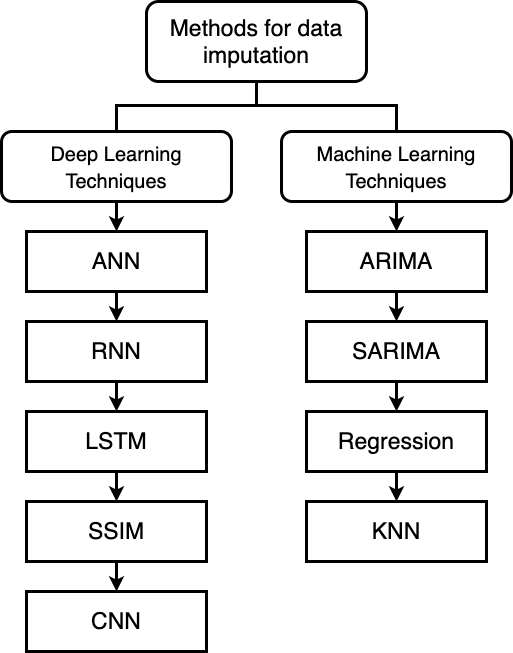
\includegraphics[width=0.5\textwidth]{images/algos.png}
	\caption{Available methods of imputation}
	\label{fig:algos}
\end{figure}

Recurrent Neural Network (RNN) - 
RNN is a machine learning technique in which temporal sequence is considered while making forecasting. Because of this reason it performs better than ANN. But still it is not capable to model upon large sequences of temporal data.\cite{26}
\\

Long Short Term Memory (LSTM) - 
The problem of remembering large sequence data and inferring upon it is overcome by LSTM network.\cite{27}
\\

Sequence to Sequence Imputation Model (SSIM) - 
In SSIM \cite{37} instead of predicting just the next data point in the sequence, it is capable of forecasting several data points next to the current end. Attention mechanism and (Variable length sliding window) VLSW are used for further improving the model accuracy/efficiency.\cite{28}
\\

Convolutional Neural Network (CNN) - 
The convolutional neural network is a technique in machine learning which is very famous in the image processing and video processing field. As it tries to learn the spatial arrangement of the pattern it proves to be useful in time series forecasting. But as it very resources heavy it may  not be suitable for IoT.\cite{29}
\\

\section{Summary}
Many machine learning and deep learning methods are available in the literature and can be used for making time series imputation and forecasting. Deep learning requires a large dataset to solve the problem effectively. WSN doesn't provide much data in the real-time scenario. There is also the limitation of applying deep learning of the scratch on end nodes due to low computing power and low memory available in the sensing nodes.

\chapter{Prelimnary Techniques}
%!TEX root = ../main.tex
\section{Overview}
This chapter provides various tools and techniques that are used in this thesis like VLSW protocol used, SSIM model used and other language and framework details and platform used for realisation of the techniques proposed by this thesis.

\section{VLSW Protocol}
Variable-length sliding window protocol is a technique to generate time-series data for training machine learning or deep learning model. In this technique, a window of variable length is moved over the data, with zero-padding the remaining unaddressed bits of the window. For time series imputation of five consecutive timestamps, the variable-length window before and after that timestamp is collected and stacked into an array of data, and the actual values of that five timestamp data are used as the output of the algorithm. Figure \ref{fig:vlsw} describes the working of variable length sliding window protocol.

\begin{figure}[ht]
	\centering
	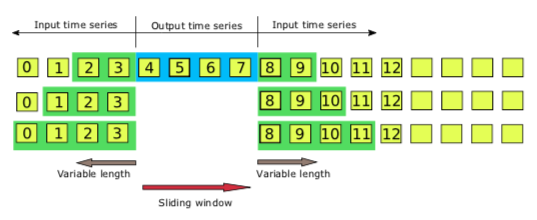
\includegraphics[width=0.8\textwidth]{images/vlsw.png}
	\caption{VLSW Protocol}
	\label{fig:vlsw}
\end{figure}

\section{Sequence to Sequence Imputation Model}
SSIM model module consist of 4 processes which are:
\begin{itemize}
\item Encoder
\item Attention layer
\item Decoder
\item Dense layer
\end{itemize}

\begin{figure}[ht]
	\centering
	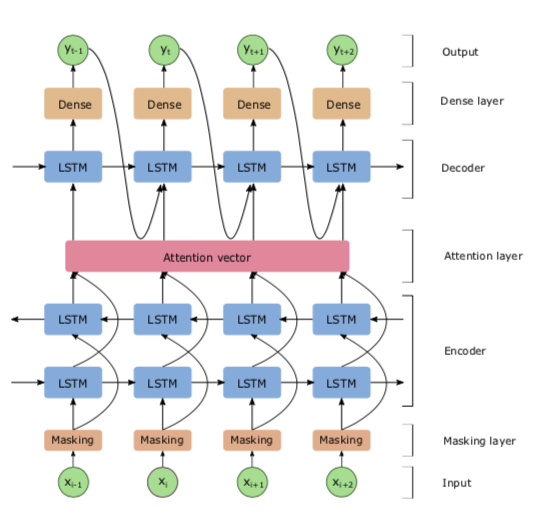
\includegraphics[width=0.5\textwidth]{images/ssim.png}
	\caption{SSIM Model Architecture}
	\label{fig:ssim}
\end{figure}

BiLSTM is used as the encoder which processes the data sequence in both directions i.e in forward direction and in backward direction. It checks for the pattern and learns its attention mechanism that  is used to focus on a specific part of the sequence which is necessary to generate the output sequence. Figure. \ref{fig:ssim} describes the SSIM model architecture.


\section{Implementation Tools}
Following is the disscussion about the tools that are used for implementing the models and training and testing the approach.

\subsection{Python}
Python is an interpreted, high-level, general-purpose programming language. It is widely used for programming machine, and deep learning algorithms, many famous machine learning, and deep learning libraries are built into python. Data scientists and data analysts widely use them. Prototyping is very easy in this language, and it is easy to learn and master. It is best suited for training deep learning models. The very famous deep learning framework Tensorflow is built using this language.

\subsection{Scikit Learn}
Scikit learn is a free opensource machine learning library written in python language. There may machine learning algorithms are implemented into this library like classification, regression, and clustering algorithms, including support vector machines, random forests, gradient boosting, k-means, and DBSCAN, and is designed to interoperate with the Python numerical and scientific libraries NumPy and SciPy. There are many helper functions and machine learning useful methods are implemented that can be used out of the box.

\subsection{Tensorflow}
Tensorflow is a software application popular for implementing machine learning algorithms, particularly neural networks. It was developed by Google it was released as an open-source platform in 2015. It is called Tensorflow because it takes input as a multidimensional array. Multidimensional arrays are also known as tensors you can construct a sort of flow chart of operation you want to perform on that input so input goes in at one end, and then it flows through this system of operation and comes out the other end as output, and that is why it is called TensorFlow. It's extremely versatile; it can be run on many diff platforms (computers, pc, laptops, raspberry pi, etc.). It can be trained on multiple machines. It can also run on GPU as well as CPU. There is tensorboard to help monitor the operation of machine learning algorithms visually.  

\subsection{Pandas}
Pandas is a python library that gives a great set of tools for data analysis. With pandas you can load prepare manipulate model and analyze data, can join data, reshape data, merge data, Combine datasets. It is very useful library for data manipulation. In this thesis the pandas is used to wrangel the dataset remove missing values and padding and careing the timestamps so that can be made in sequence manner so that deep learning algorithms can be applied to it.
\\

\subsection{Matplotlib}
Matplotlib is a tool for data visualization in python strongly coherred with numpy and pandas. It helped in the thesis for generating the result graphs and other graphs needed for the analysis.
\\

\subsection{Google Colab}
Google Colab is a Jupyter notebook in the google cloud pre installed with many machine learning and deep learning libraries generally needed for the data analysis data visualization, machine learning and deep learning. Beside that other not installed libraries can also be installed and used. It also provide the GPU (Graphics Processing Unit) support for training the models very fast as compared to CPU (Centeral Processing Unit) which is also available and can be used. Along with CPU and GPUs it comes with TPU (Tensor Processing Unit) which are special kind of GPU specialy designed to work with the very famous tensorflow framework. Currently it is only available in the google cloud hosted platforms like colab or for custom google compute cloud one can easily build and run machine learning algorithms in the cloud.
\\

\section{Summary}
In this chapter various tools and techniques are described that uare used for the development of the proposed work. The next chapter describes the solution to the problem using the tools and techniques.

\chapter{Critical Analysis of Imputation Techniques}
%!TEX root = ../main.tex

\section{Overview}
In this chapter various timeseries imputation and forecasting techinques are compared and results are compiled along with their implementation details. The results of the SSIM model is also described here which is an encoder decoder model the type of model normally used in machine translation techniques.

\begin{table}[h]
	\centering
	\begin{tabular}[widht=\textwidth]{|l | l |}
	\hline
	Model & MSE Score\\
	\hline
	Regression & 0.342\\
	\hline
	LSTM & 0.094\\
	\hline
	CNN & 0.0763\\
	\hline
	SSIM & 0.0944\\
	\hline
	\end{tabular}
	\caption{Comparision of time series techniques}
	\label{tab:technique-comparision-table}
\end{table}

\section{Regression}
Regression is a the core of most of the machine learning algorithm. For time series imputation regression technique can be used although it may not give the best results but it gives the fairly satisfiable results based on time taken by the algorithm to make a prediction model.

\begin{figure}[ht]
	\centering
	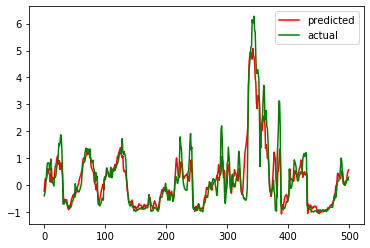
\includegraphics[width=0.8\textwidth]{images/techniques/regression.png}
	\caption{Regression PM2.5 Actual vs Predicted graph}
	\label{fig:regression-tech}
\end{figure}

 Figure \ref{fig:regression-tech} shows an actual vs predicted graph of the a regression model trained on the PM2.5 values of Beijing city. Table \ref{tab:technique-comparision-table} contains the MSE score achieved by the model.

\section{LSTM}
Long Short Term Memory(LSTM) Network is a special kind of recurrent neural network where it maintain a cell state variable which helps it to deal with the vanishing gradient problem in RNNs. It proves to be making it very feasible for time series imputation.


\begin{figure}[ht]
	\centering
	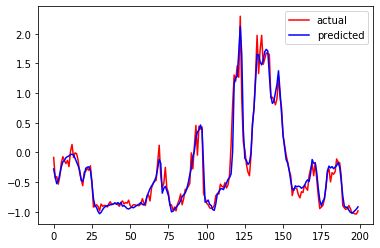
\includegraphics[width=0.8\textwidth]{images/techniques/lstm.png}
	\caption{LSTM PM2.5 Actual vs Predicted graph}
	\label{fig:lstm-tech}
\end{figure}


An LSTM model is trained on PM2.5 its MSE score is listed in table \ref{tab:technique-comparision-table}. Figure \ref{fig:lstm-tech} shows the actual vs predicted graph of the LSTM model trained on the PM2.5 values of Beijing city.

\section{CNN}
Convolutional Neural Network is very famous neural network for the field of image recognition and computer vision. It has feature of pattern detection which makes it very feasible in time series forecasting as in time series forecasting and imputation certain pattern in the data need to be exploited for making the prediction. It is generaly used with non covolutional layers in the deep learning but the main core of it is the convolutional layer which are responsible for exploiting the pattern in the data.

\begin{figure}[ht]
	\centering
	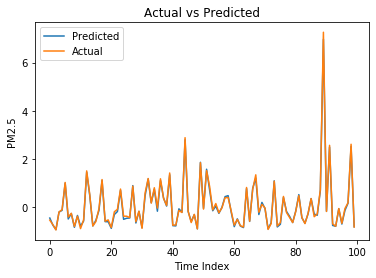
\includegraphics[width=0.8\textwidth]{images/techniques/cnn.png}
	\caption{CNN PM2.5 Actual vs Predicted graph}
	\label{fig:cnn-tech}
\end{figure}

Figure \ref{fig:cnn-tech} show the actual vs predicted graph of the CNN model trained on PM2.5 values of beijing city. Table \ref{tab:technique-comparision-table} show list the MSE score of the model.

\section{SSIM}
Sequence to Sequence Imputation Model (SSIM) is an encoder decoder model using the LSTM model as encoder attention vector is used which the encoder convert the input sequence into and another LSTM model is used as the decoder model after that a dense layer is also used for softmax values of the sequence to be generated. The working of the encoder decoder model is such that a variable length input is given to the network it converts the given input sequence to a fixed length vector known as attention vector, and the decoder convert the attention vector into the desired length sequence vector for the output.

\begin{figure}[ht]
	\centering
	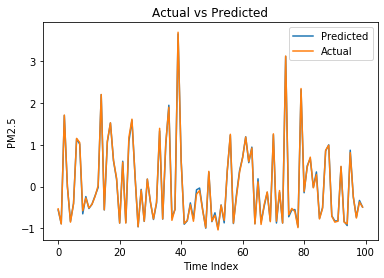
\includegraphics[width=0.8\textwidth]{images/techniques/ssim.png}
	\caption{SSIM PM2.5 Actual vs Predicted graph}
	\label{fig:ssim-tech}
\end{figure}

Figure \ref{fig:cnn-tech} show the actual vs predicted graph of the SSIM model trained on PM2.5 values of beijing city. Table \ref{tab:technique-comparision-table} show list the MSE score of the model.

\section{Summary}
In this cahpter various available machine learning and deep learning models are implemented and their mse score and actual vs predicted graphs are compared. All these model works well when they are applied on some problems where there are properly large amount of data available. In the next chapter a new approach of dealing with problem when not much data is available with hand the how deep learning models can be applied. The Transfer Learning For Time Series Imputation is applied on the two deep learning models which works well with time series problem i.e., CNN and SSIM. 

\chapter{Proposed Work}
%!TEX root = ../main.tex

% Name of the model: Transfer Learning For Time Series Imputation
\section{Overview}
In this chapter the proposed work of \textbf{Transfer Learning For Time Series Imputation} is described with the system models, analytical models, flow diagrams, model architecture, trained model symmary along with the discussion about every components in detail.

\section{System Model}

System model is such that once we achive the desired level of model accuracy and loss value that model are deployed in the real environment so that it get used and also trained in online environment which is that it self correct and make the system self sufficient .Our system model consists of the following components.

\subsection{Sensing Layer}
Sensors and actuators in this layer collect data from the environment in this layer.
Also, it provides the interface to the real world to interact with the environment and provide impact in the physical world. It helps in both collecting data from the environment and to provide action that results in the making system work properly with in the sync.

\subsection{Network Layer}
Data collected by the sensing layer is transported to the computing devices and processing and control system using Network Layer. This layer is used for transporting the processed and to be processed data to and fro from on end to the other end. Many protocols and networks like MQTT COAP can be used easily.

\subsection{Data Processing Layer}
The data processing layer is the layer of IoT Architecture where all the computing of the system occurs. Our paper tries to solve the problem all of which lies here. It is the part of processing unit as shown in Figure. \ref{fig:system-model}

\underline{Nature of IoT data} - IoT systems generates high-volume, streaming, location, and time-specific this type of data is called time-series data. 
We would be deploying our fault-tolerance system in this layer only.

\subsubsection{Fault tolerance layer}
In this layer, we predict the missing values that our sensors don’t able to collect. This may be due to many various reasons like sensor failure, network disturbance, battery discharge etc. this is the part where the action according to the predictions is taken. It may be some alarm initiation some improvement logic or simply update the record in the database. This is also the part of the processing unit as shown in Figure. \ref{fig:system-model}

\subsection{Application layer}
The application layer is the layer where the user interacts with the system or the machine interface takes action based on the output of the IoT system. 

Application layer can be made in any framework that working and nature of problem. In the current simulation scenario as the pollution data is taken for the reference it is more feasble to make a web interface where an user can see the real time monioring of the various weather and pollution parameters and if required can take action based on the results shown in the dashboard. For making the dashboard any front end framework can be used like Angular or React where it is very easy to build user interfaces with single page application. For the backend python framework like django or flask can be used as it will help in predicting and implementing the machine learning models on the cloud environment.
\\
Server side application programmable interface and front end dashboard can be connected with the any real time network interface. The one which would work feasible is socket. Other protocols like MQTT or COAP can also be used.

In the fault tolerance layer, we have generated a machine learning model in that we can generate inferences from and also train the model in real-time.




\begin{figure}[ht]
	\centering
	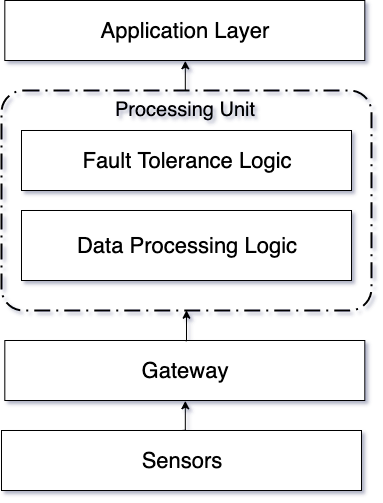
\includegraphics[width=0.5\textwidth]{images/system-model.png}
	\caption{System Model}
	\label{fig:system-model}
\end{figure}

\section{System Flow}
In this section the flow of the data and precessing and imputation processes are described. The figure \ref{fig:system-flow-diagram} dipicts the system flow diagram in the form of data flow diagram.

\begin{figure}[ht]
	\centering
	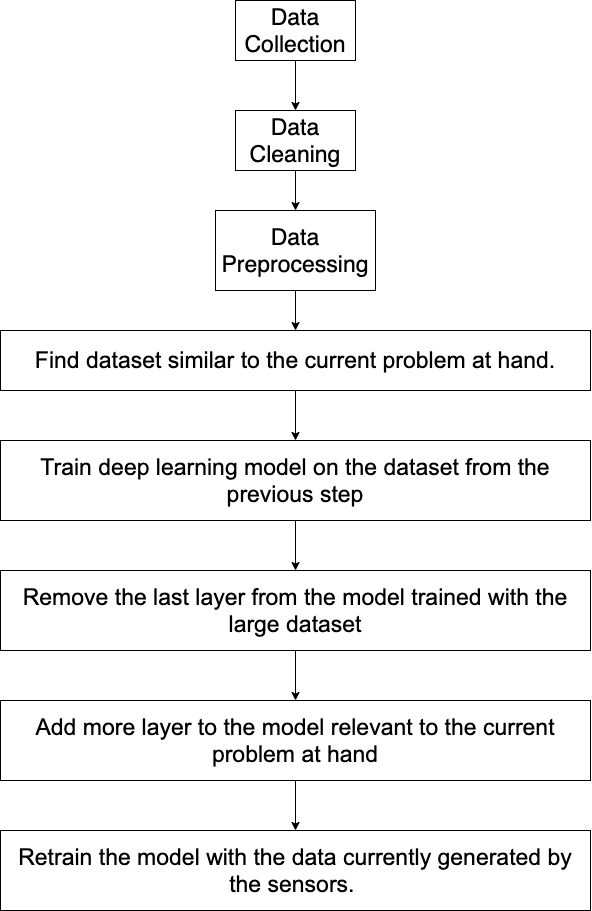
\includegraphics[width=0.8\textwidth]{images/system-flow-diagram.png}
	\caption{System Flow Diagram of Transfer Learning For Time Series Imputation}
	\label{fig:system-flow-diagram}
\end{figure}




\subsection{Data Collection}

For this demonstration and testing the approach proposed 
PM2.5 Data of two chinese are taken. This data is taken from UCI machine learning repository. It is very famous source for dataset for academic purposes. It contains many famous machine learning dataset widely used for academic and research perposes. Some of them are IRIS Flower Dataset, Titanic Survival dataset, etc. The two cities PM2.5 values data are taken from a dataset containing PM2.5 values of five chinese cities named "PM2.5 Data of Five Chinese Cities Data Set". Description of the dataset used is given below.

\underline{Dataset abstract} This hourly data set contains the PM2.5 data in Beijing, Shanghai, Guangzhou, Chengdu and Shenyang. Meanwhile, meteorological data for each city are also included.

The table \ref{tab:dataset-characteristic} describe the nature of the dataset.

\begin{table}[ht]
\centering
\begin{tabular}[widht=\textwidth]{|l|l|}
\hline
Data Set Characteristics &  Multivariate, Time-Series \\
Number of Instances & 52854 \\
Area & Physical \\
Attribute Characteristics & Integer, Real \\
Number of Attributes & 86 \\
Date Donated & 2017-07-18 \\
Associated Tasks & Regression \\
Missing Values? & Yes \\
Number of Web Hits & 81692 \\
\hline

\end{tabular}
\caption{Dataset Characteristics}
\label{tab:dataset-characteristic}
\end{table}

The table \ref{tab:dataset-attributes} describe attributes and features of the attributes of the dataset.


% Feature Table
\begin{table}[ht]
\centering
\begin{tabular}[widht=\textwidth]{|l|l|}
\hline

No & row number \\
year & year of data in this row \\
month & month of data in this row \\
day & day of data in this row \\
hour & hour of data in this row \\
season & season of data in this row \\
PM & PM2.5 concentration  \\
DEWP & Dew Point (Celsius Degree) \\
TEMP & Temperature (Celsius Degree) \\
HUMI & Humidity (\%) \\
PRES & Pressure (hPa) \\
cbwd & Combined wind direction \\
Iws & Cumulated wind speed (m/s) \\
precipitation & hourly precipitation (mm) \\
Iprec & Cumulated precipitation (mm) \\
\hline
\end{tabular}
\caption{Dataset Attributes}
\label{tab:dataset-attributes}
\end{table}

The two cities selected out of 5 are Beijing and Shanghai. Beijing data is used as the data set with large values and the Shanghai data is considered as the realtime data for which deep learning model need to be developed. This data is traind both without using transfer learning and with the transfer learning applied.

\subsection{Data Cleaning}

Data cleaning is a process of sanitising the data available with us so that its usabilituy may increase. There is a very famous phrase in data science garbage in garbage out. So data cleaning is very important step in any data related work.

Dataset contains many missing values which currently cannot make use of as it is so the missing values columns are dropped from the dataset managing the consistency in the dataset and the cleaned datase is used for the further processing.

Following method of the pandas is used for the cleaning the data.

\begin{verbatim}
pm25_beijing = df1.iloc[:, 5].dropna().values[:].reshape(-1, 1)

pm25_shanghai = df2.iloc[:, 9].dropna().values[:600].reshape(-1, 1)
\end{verbatim}

\subsection{Data Preprocessing}

\subsubsection{Loading the data}
The dataset is stored on a github repository so that it can be easily accessed through a link anywhere the code is running. The only need would be internet access while runing the code.

Matplotlib library is used for loading the data in the python environment. 

\begin{verbatim}
import matplotlib.pyplot as plt
URL_beijing = "LINK_OF_GITHUB_CSV_FILE"
df_beijing = pd.read_csv(URL_beijing)
\end{verbatim}

\subsubsection{Removing unnecessary data}
Actually the dataset consisted of various featue about the weather but for simplicity all other attributes except PM2.5 were removed.

\subsubsection{Scaling the data}
The PM2.5 values are not in the range of -1 to 1 so these values are scaled down to -1 to 1 range so that the can be fed to the machine learning algorithm later.

Scikit learn StandardScaler function is used for scaling the data down.

\begin{verbatim}
from sklearn.preprocessing import StandardScaler
scaler_beijing = StandardScaler()
scaler_beijing.fit(pm25_beijing)
pm25_beijing = scaler_beijing.transform(pm25_beijing)
\end{verbatim}

\subsubsection{Making dataset as input output pair for training}

There are several ways of doing this the one best technique of doing this. One method is discussed earlier.
For this sliding window protocol is used for making this data as supervised learning dataset so that it can be trained.

\begin{verbatim}
N = 20
O = 5
P = 20

X_beijing = []
y_beijing = []

for i in range(len(pm25_beijing) - (N + O + P)):
    temp = []
    temp1 = pm25_beijing[i : i+N]
    temp2 = [0 for _ in range(O)]
    temp3 = pm25_beijing[i+N+O : i+N+O+P]
    X_beijing.append(np.append(np.append(temp1, temp2), temp3))
    y_beijing.append(pm25_beijing[i+N : i+N+O].reshape(O))
\end{verbatim}


Here N is the length of the left slide length, O is the output length, i.e., for how many timestamp we want to predict the output, and P is the length of the right slide length.

The X data is prepared as to consist of left slide length from the sequence of data available for the output lenth 0 is filled in the sequence and at last the right slide length data is attached.

The y of the dataset is prepared by taking the actual values of the timestamp values of the O length datapoints.


\subsection{Finding Similar Dataset}
As the transfer learning to work for the WSN or IOT data it is necessary to find some dataset similar to the problem at hand that need to be solved. This type of cases can be very simmilar to real world such that a new thermal plant is need to be installed in any area and there is need for some fault toulerence logic for that but not have enough data to train the deep learning model for that. For that similar dataset can be picked from any similar thermal plant sensors.

For training for the shanghai PM2.5 value prediction Beijing data is used as training point for applying the transfer learning.

\subsection{Training deep neural network}

\subsubsection{Spliting the dataset into training and test sets}
Before feeding the data to the model the first step is to split the data into training and the test set so that model performance can be measured.\\

Scikit-Learn library model selection model train test split function is used for spliting the dataset into the training and testing values.\\

Code for this splitting is provided below\\

\begin{verbatim}
from sklearn.model_selection import train_test_split
X_train, X_test, y_train, y_test = train_test_split(X_beijing, y_beijing)
\end{verbatim}
\subsubsection{Training}

The first step of applying transfer learning is to train the model with huge amount of data available from any source which give the huge amount of data. The dataset for transfer learning training is picked in the previous section, that is Beijing city data. The deep learning model is first trained on the Beijing PM2.5 values dataset that contains data from previous several years.

\subsection{Removing last layer of DNN}
For applying the transfer learning to with the existing model the first step is to remove the last layer of the trained model so that new model with its features and attributes can be coded. the main motive of removing the last layers of the DNN to apply transfer learning is to incorporate the feature of the dataset one we are trying to train now.

\subsection{Adding more layer to the DNN}
The next step of applying the trasfer learning is to add more layer to the model from the previous step so that the new feature can be incorporated and trained again for the new dataset. 

*Note: The last two steps can be ignored if nature and nature of data is ditto same.

\subsection{Retraining the model}
When new layer is added to the model now it can be trained on the data available now for new sensor on new location. Training can be in any manner, i.e., online training or batch training.

\section{Model Architecture}

The two models is selected for applying transfer learnig for this proposed work. Figure \ref{fig:model-summary} describes the model summary of the two models.

\subsection{SSIM (Sequence to Sequence Imputation Model)}

	LSTM is a special kind of RNN(Recurrent Neural Network) which exploit the pattern in the data which makes. It has a memory unit which remember the previous sequence in the memory.
	SSIM is an encoder decoder model which is generally used in natural language processing for machine translation and it can be used here for time series imputation. Figure \ref{fig:shanghai-ssim-model-summary} Describe this architecture of the SSIM model.

	The SSIM model architecture contains the followin layers.
	\subsubsection{Bidirectional LSTM layer}
	It is a bidirectional LSTM layer to exploit the data in both the direction in forward along with backwards. 

	There are 128 neurons used in the Bidirectional LSTM layer.

	\subsubsection{Attenttion Layer}
	This is a layer used in Encoder Decoder model to focus on certain specific part of the sequence which are more relevant to the application and provides better results.
	An analogy of this is found in the image processing where the task is to identify the object in the image. Since the object in the image can be found in certain part of the photograph it need to focus on that part of the photo to identify the object. Figure. \ref{fig:attention} describes this proces of attention mechanism in terms of computer vision.

	\begin{figure}[ht]
		\centering
		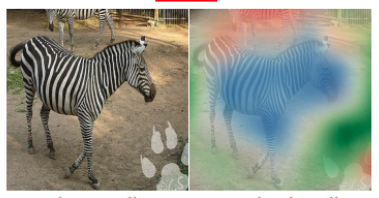
\includegraphics[width=0.8\textwidth]{images/attention.png}
		\caption{Attention Mechanism in terms of computer vision}
		\label{fig:attention}
	\end{figure}

	\subsubsection{LSTM Layer}
	This is a simple LSTM layer in the SSIM model comparising the decoder of the encoder decoder system. This layer is used for decoding the sequence generated by the input.

	\subsubsection{Dense Layer}
	This layer is used for maping the output sequence to the desired number of output timestamp values needed by the model.



\subsection{CNN (Convolutional Neural Network)}

	Convolution neural network is basically the applied in the field of image recognition and computer vision to find pattern in the image and label according to the labels given to it. Figure \ref{fig:shanghai-ssim-model-summary} describes the model summary of the CNN model.

	\subsubsection{Conv1D Layer}
		This is the first layer of the CNN model containing for learning the pattern in the data. It contains with 64 filters, kernal size is 3 and relu activation function is used.

	\subsubsection{MaxPooling Layer}
		Maxpooling layer is used to down sample input to eleminate the overfitting the training data.

	\subsubsection{Flatten Layer}
		The flatten layer is used to change the shape of the input to the 1D sequence of data.

	\subsubsection{Dense Layer X 2}
		Two Dense Layer is used one with 50 neurons and another with the 5 neurons to generate the output sequence of the desired length (5 timestamp)


\begin{figure}[ht]
	\centering
	\begin{subfigure}[b]{0.80\textwidth}
		\centering
		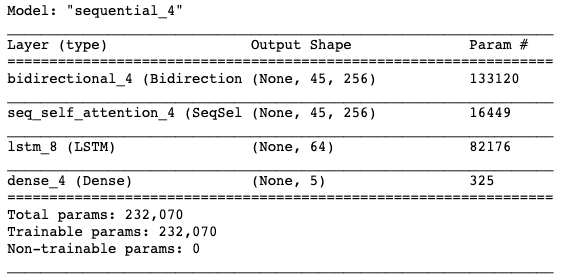
\includegraphics[width=\textwidth]{shanghai-ssim-model-summary}
		\caption{Shanghai SSIM Model Summary}
		\label{fig:shanghai-ssim-model-summary}
	\end{subfigure}
	\hfill
	\begin{subfigure}[b]{0.80\textwidth}
		\centering
		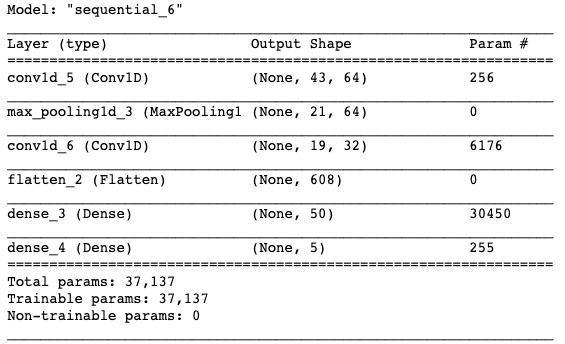
\includegraphics[width=\textwidth]{shanghai-cnn-model-summary}
		\caption{Shanghai CNN Model Summary}
		\label{fig:shanghai-cnn-model-summary}
	\end{subfigure}
	\caption{Model summary of transfer learning}
	\label{fig:model-summary}
\end{figure}

\section{Summary}
In this chapter the working of the whole proposed system is discussed in details. In the next chapter the results generated by the system is analysed and described in details.

\chapter{Results and Analysis}
%!TEX root = ../main.tex

In the previous chapter the proposed work is explained in details. In this chapter the results generated by applying transfer learning on the shanghai data with two models, SSIM and CNN is analysed.


% \begin{figure}[ht]
% 	\centering
% 	\begin{subfigure}[b]{0.7\textwidth}
% 		\centering
% 		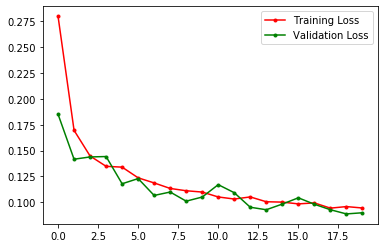
\includegraphics[width=\textwidth]{beijing-ssim-training}
% 		\caption{Beijing SSIM}
% 		\label{fig:beijing-ssim-training}
% 	\end{subfigure}
% 	\hfill
% 	\begin{subfigure}[b]{0.7\textwidth}
% 		\centering
% 		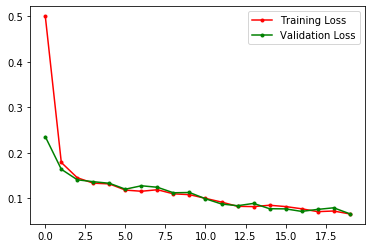
\includegraphics[width=\textwidth]{shanghai-ssim-training}
% 		\caption{Shanghai SSIM}
% 		\label{fig:shanghai-ssim-training}
% 	\end{subfigure}
% 	\hfill
% 	\begin{subfigure}[b]{0.7\textwidth}
% 		\centering
% 		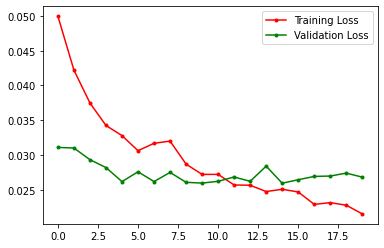
\includegraphics[width=\textwidth]{shanghai-ssim-transfer-learning}
% 		\caption{Shanghai SSIM Transfer Learning}
% 		\label{fig:shanghai-ssim-transfer-learning}
% 	\end{subfigure}
% 	\caption{Comparision of loss graph in applying transfer learning in SSIM}
% 	\label{fig:}
% \end{figure}


\begin{table}[h]
\centering
\begin{tabular}[widht=\textwidth]{|l | l | l | l | l|}
\hline
 & Beijing data & Shanghai data  & Shanghai with TL & Improvement \\
\hline
CNN & 0.0763 & 0.031 & 0.015 & 52 \% \\

SSIM & 0.0944 & 0.0656 & 0.0215 & 67 \% \\
\hline
\end{tabular}
\caption{Comparision of MSE Loss of various model with transfer learning}
\label{tab:comparision-table}
\end{table}


\textbf{MSE Loss}
MSE (Mean Squared Error) is the loss function that is used for the training the models on the sensor data. It is used to measure the efficienty of the model trained. Lesser the value of MSE score more the model is efficient. \\

\begin{figure}[ht]
	\centering
	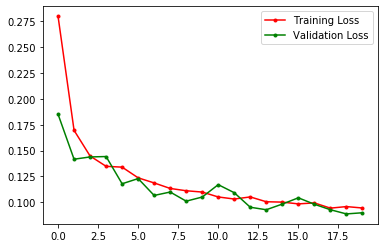
\includegraphics[width=0.8\textwidth]{beijing-ssim-training}
	\caption{Beijing SSIM}
	\label{fig:beijing-ssim-training}
\end{figure}


\textbf{Beijing data on CNN model}
On training CNN model with bejing data mse score achived is 0.763 \\

\textbf{Beijing data on SSIM model}
On training SSIM model with beijing data mse score achieved is 0.0944 \\

This results that SSIM model achieved more efficiency in comparision to CNN model for time series frecasting problem.\\



\begin{figure}[ht]
	\centering
	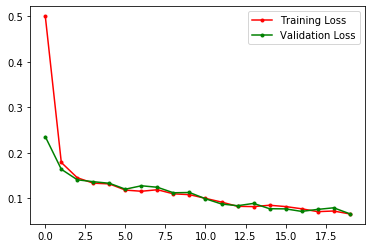
\includegraphics[width=0.8\textwidth]{shanghai-ssim-training}
	\caption{Shanghai SSIM}
	\label{fig:shanghai-ssim-training}
\end{figure}

\textbf{Shanghai data on SSIM without Transfer Learning}
On training SSIM model with shanghai data without Transfer learning mse score achieved is 0.0656\\

\textbf{Shanghai data on SSIM with Transfer Learning}
On training SSIM model with shanghai data with Transfer learning with using pretrained model of beijing data mse score achieved is 0.0215 \\

\begin{figure}[ht]
	\centering
	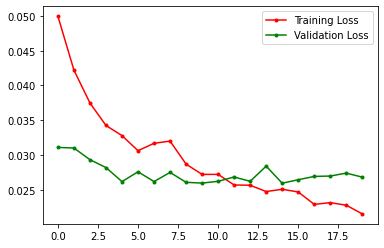
\includegraphics[width=0.8\textwidth]{shanghai-ssim-transfer-learning}
	\caption{Shanghai SSIM Transfer Learning}
	\label{fig:shanghai-ssim-transfer-learning}
\end{figure}


This results that SSIM model with transfer learning shows 67\% improvement. \\

Figure \ref{fig:beijing-ssim-training} shows the training vs validation loss graph of Beijing SSIM training \\

Figure \ref{fig:shanghai-ssim-training} show the training vs validation loss graph of Shanghai SSIM training \\

Figure \ref{fig:shanghai-ssim-transfer-learning} shows the training vs validation loss graph of Shanghai SSIM training with transfer learning with using pretrained bejing ssim model. \\

Table \ref{tab:comparision-table} Summarises all the models losses and imporvements. \\

While using SSIM model there is 67\% imporvement with transfer learning.\\

Also\\

While using CNN model there is 52\% improvement with transfer learning. \\








\chapter{Conclusion}
%!TEX root = ../main.tex
The proposed model of using transfer learning in wireless sensor network data increases the effeciency of the forecasting and imputation. It also reduces the training time which makes it more feasible for online training and for real-time scenario.\\

The result in the previous chapter shows that it make more feasible to train such model with transfer learning in comparision to the building one from scratch. MSE loss shows that more accuracy can be achieved with less data where WSN is not generating much data for applying the deep learning.


\appendix
\chapter{Screenshots of Implementation}
%!TEX root = ../main.tex

\begin{figure}[ht]
	\centering
	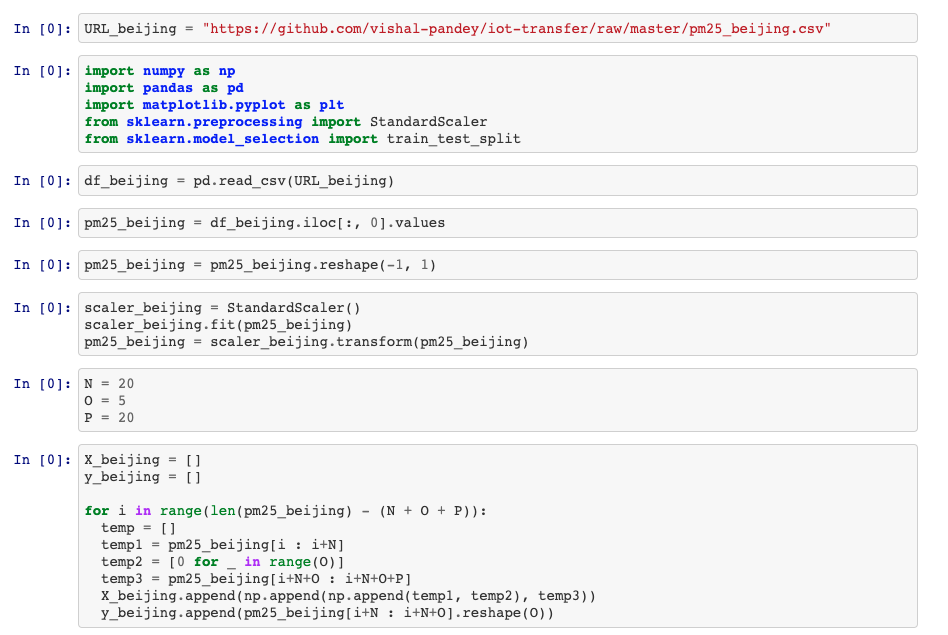
\includegraphics[width=\textwidth]{code/1}
	\caption{Code Screenshot 1}
	\label{fig:code1}
\end{figure}

\begin{figure}[ht]
	\centering
	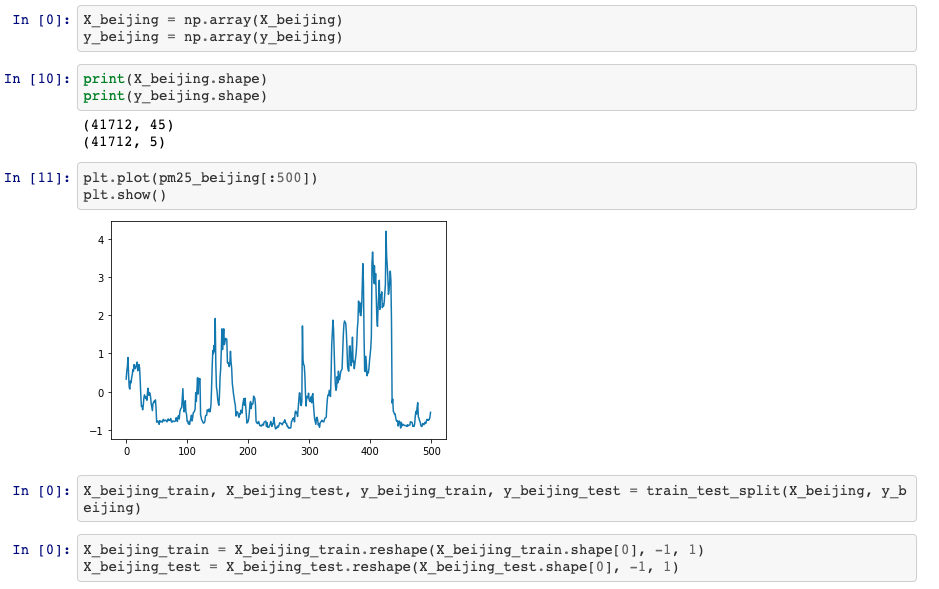
\includegraphics[width=\textwidth]{code/2}
	\caption{Code Screenshot 2}
	\label{fig:code2}
\end{figure}

\begin{figure}[ht]
	\centering
	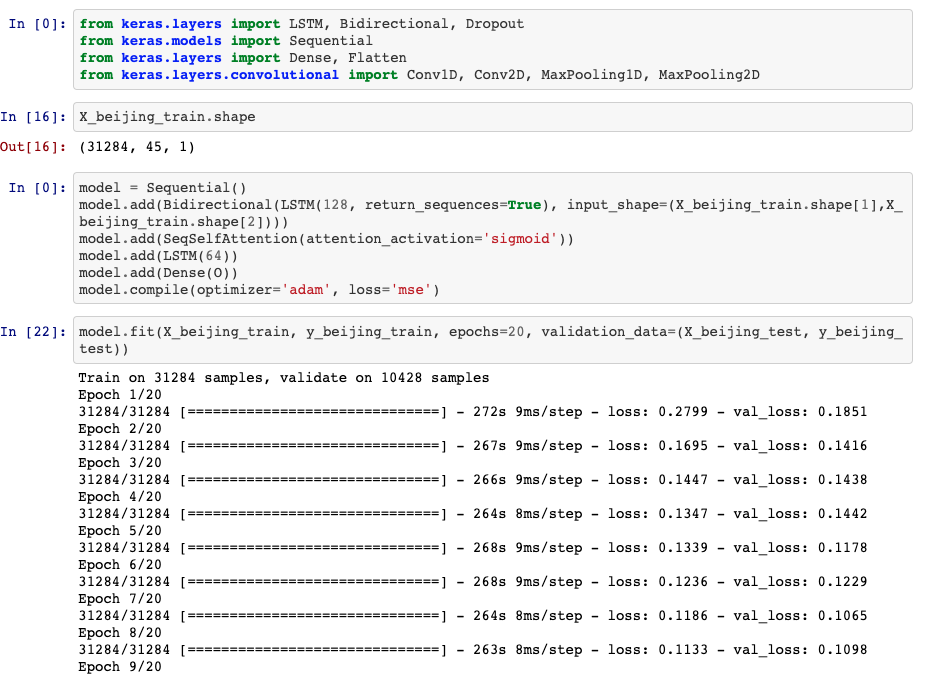
\includegraphics[width=\textwidth]{code/3}
	\caption{Code Screenshot 3}
	\label{fig:code3}
\end{figure}

\begin{figure}[ht]
	\centering
	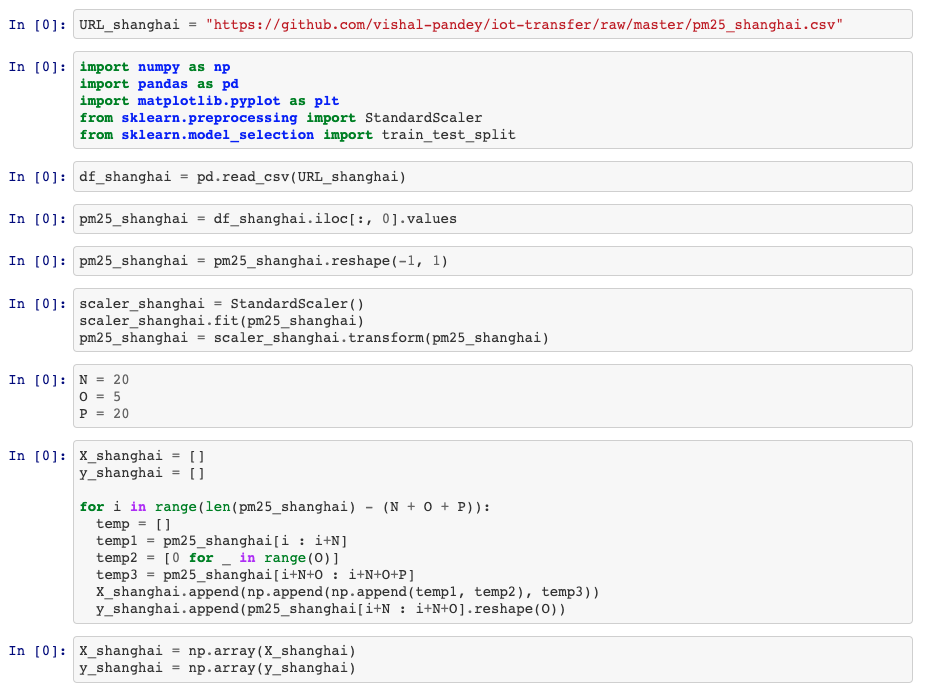
\includegraphics[width=\textwidth]{code/4}
	\caption{Code Screenshot 4}
	\label{fig:code4}
\end{figure}

\begin{figure}[ht]
	\centering
	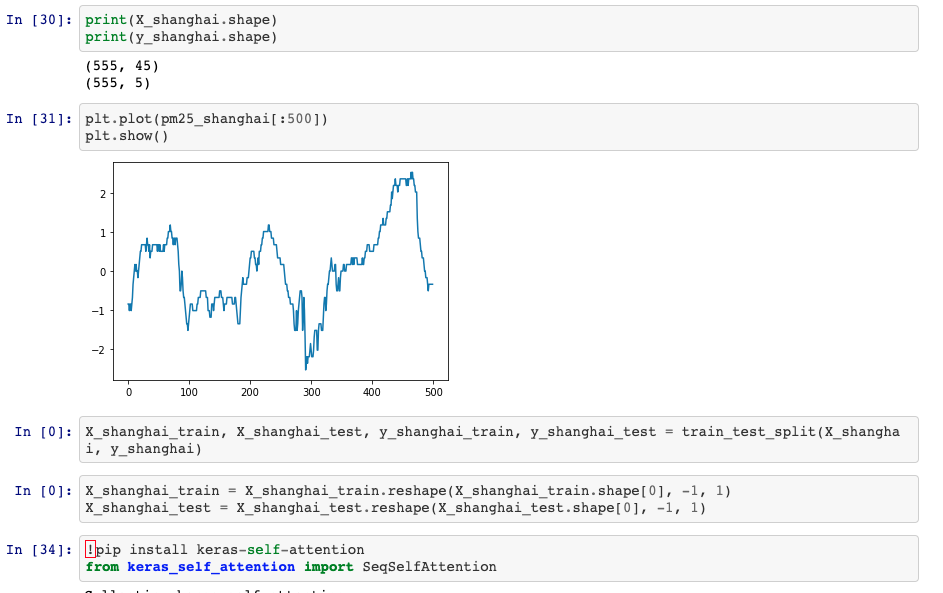
\includegraphics[width=\textwidth]{code/5}
	\caption{Code Screenshot 5}
	\label{fig:code5}
\end{figure}

\begin{figure}[ht]
	\centering
	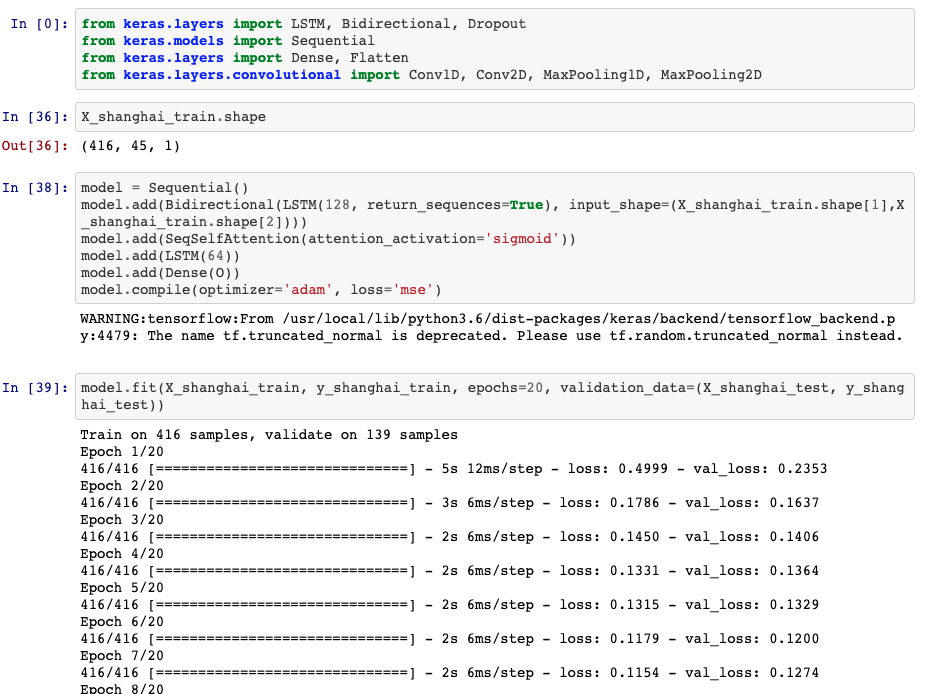
\includegraphics[width=\textwidth]{code/6}
	\caption{Code Screenshot 6}
	\label{fig:code6}
\end{figure}

\begin{figure}[ht]
	\centering
	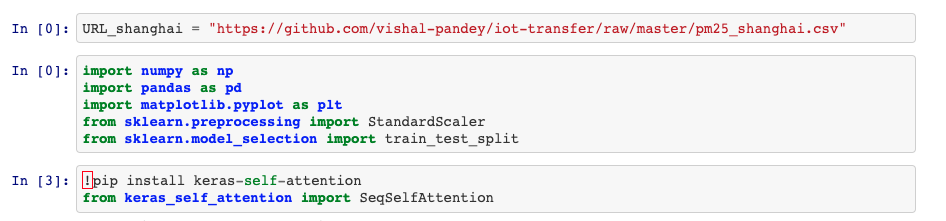
\includegraphics[width=\textwidth]{code/7}
	\caption{Code Screenshot 7}
	\label{fig:code7}
\end{figure}

\begin{figure}[ht]
	\centering
	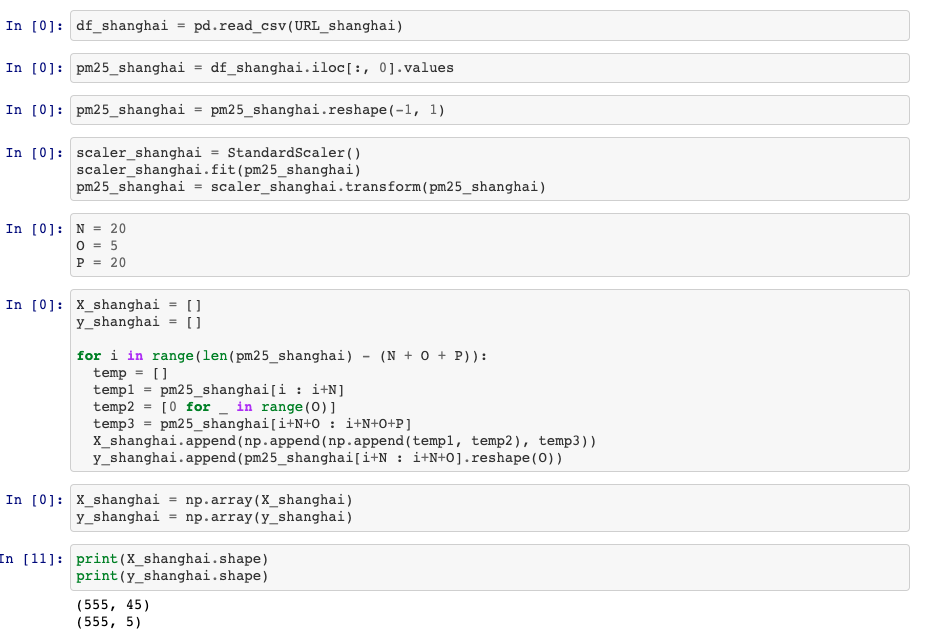
\includegraphics[width=\textwidth]{code/8}
	\caption{Code Screenshot 8}
	\label{fig:code8}
\end{figure}

\begin{figure}[ht]
	\centering
	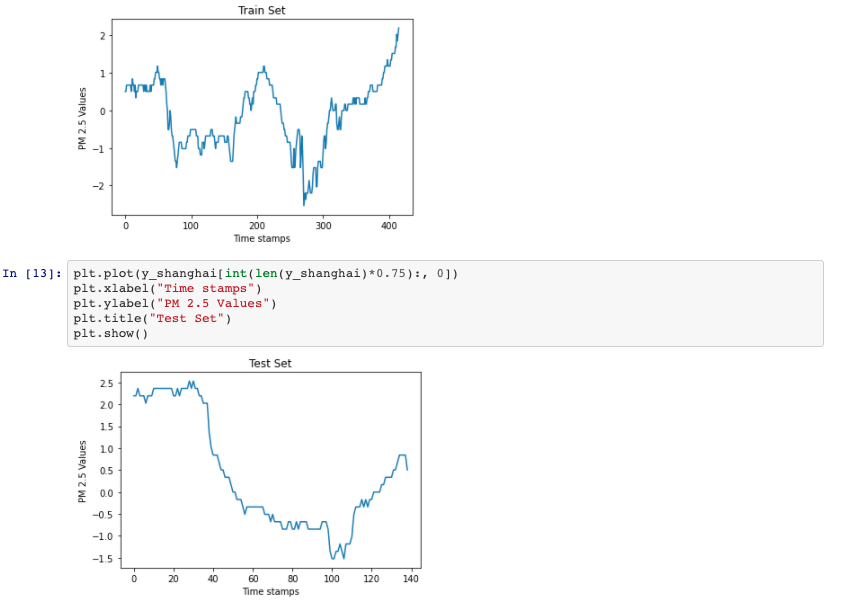
\includegraphics[width=\textwidth]{code/9}
	\caption{Code Screenshot 9}
	\label{fig:code9}
\end{figure}

\begin{figure}[ht]
	\centering
	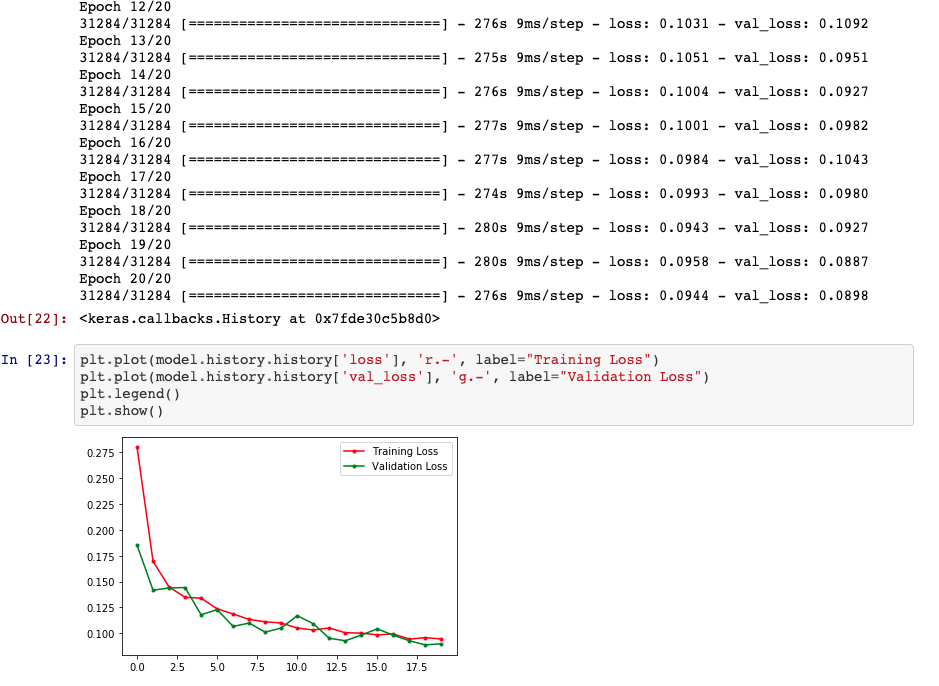
\includegraphics[width=\textwidth]{code/10}
	\caption{Code Screenshot 10}
	\label{fig:code10}
\end{figure}

\begin{figure}[ht]
	\centering
	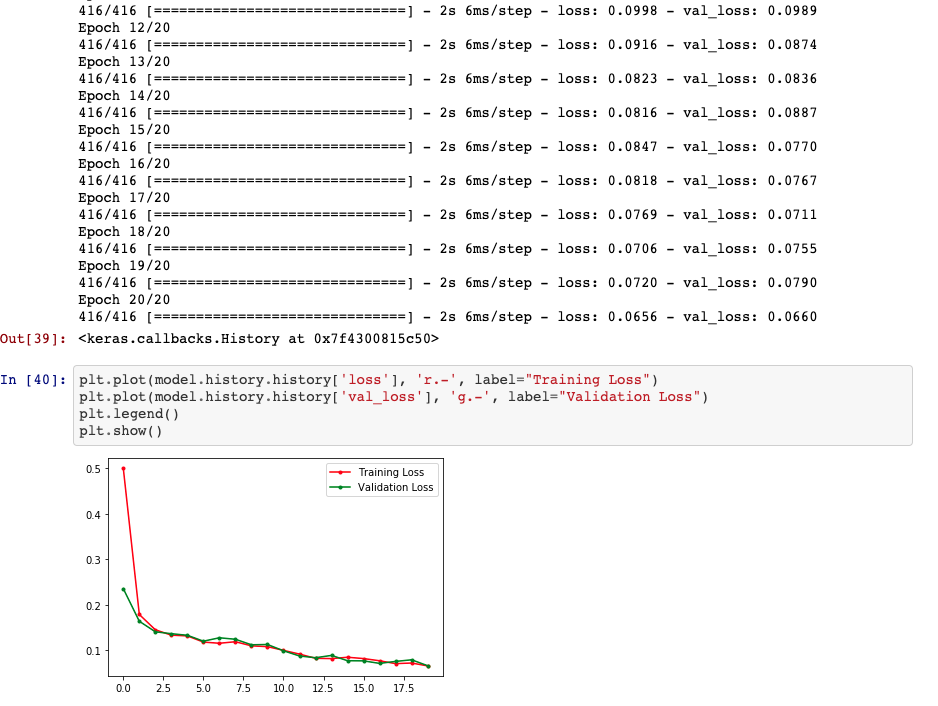
\includegraphics[width=\textwidth]{code/11}
	\caption{Code Screenshot 11}
	\label{fig:code11}
\end{figure}

\begin{figure}[ht]
	\centering
	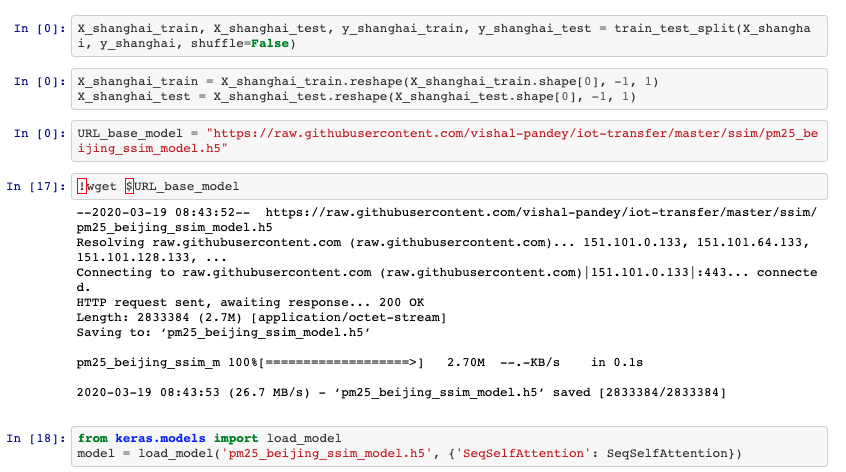
\includegraphics[width=\textwidth]{code/12}
	\caption{Code Screenshot 12}
	\label{fig:code12}
\end{figure}

\begin{figure}[ht]
	\centering
	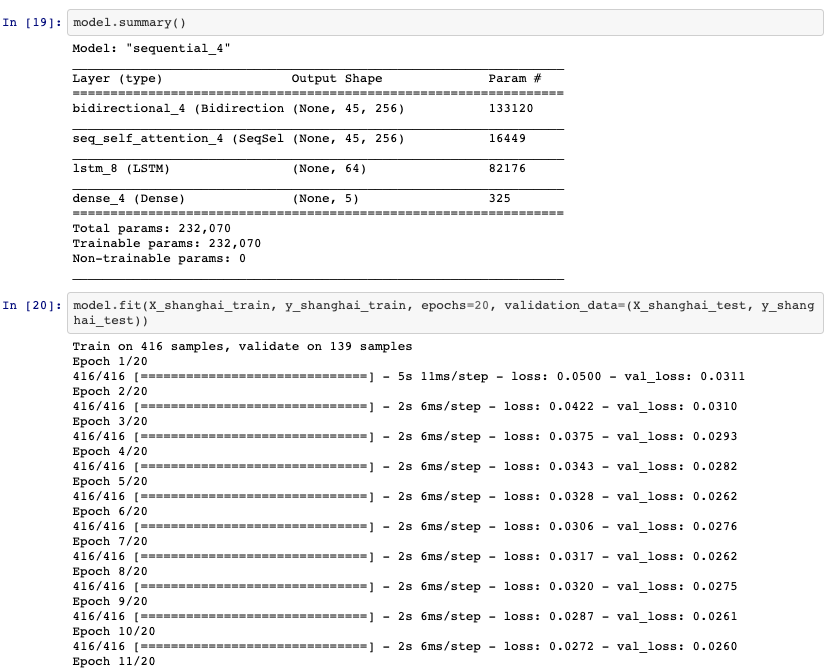
\includegraphics[width=\textwidth]{code/13}
	\caption{Code Screenshot 13}
	\label{fig:code13}
\end{figure}

\begin{figure}[ht]
	\centering
	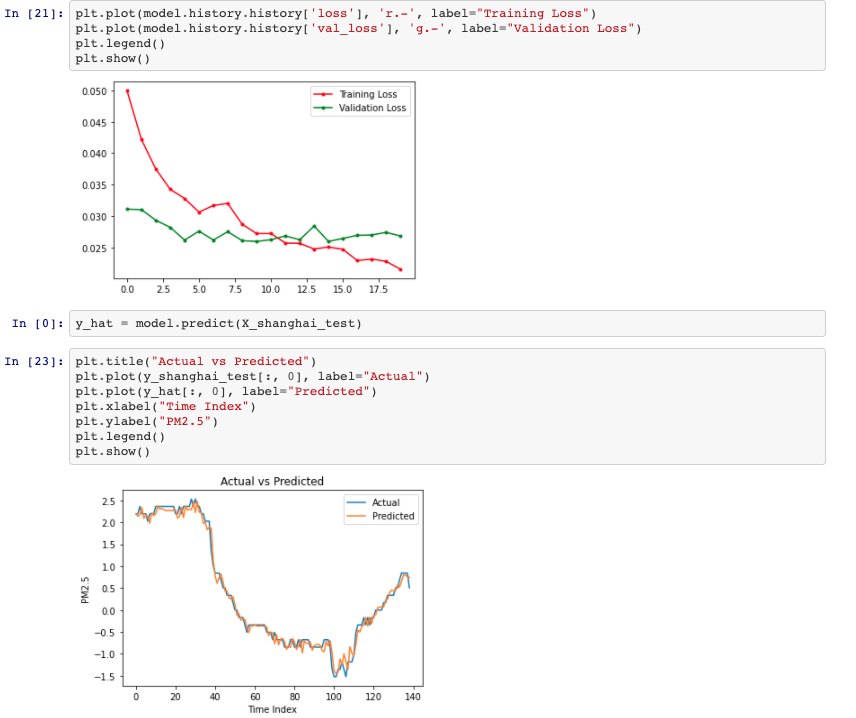
\includegraphics[width=\textwidth]{code/14}
	\caption{Code Screenshot 14}
	\label{fig:code14}
\end{figure}



\begin{thebibliography}{}

\bibitem{1}[M. Mousa, M. Abdulaal, S. Boyles and C. Claudel, "Wireless Sensor Network-Based Urban Traffic Monitoring Using Inertial Reference Data," 2015 International Conference on Distributed Computing in Sensor Systems, Fortaleza, 2015, pp. 206-207, doi: 10.1109/DCOSS.2015.21.

\bibitem{2}[H. Furtado and R. Trobec, "Applications of wireless sensors in medicine," 2011 Proceedings of the 34th International Convention MIPRO, Opatija, 2011, pp. 257-261.

\bibitem{3}[Bardella, A., Danieletto, M., Menegatti, E. et al. Autonomous robot exploration in smart environments exploiting wireless sensors and visual features. Ann. Telecommun. 67, 297–311 (2012). https://doi.org/10.1007/s12243-012-0305-z

\bibitem{4}[M. R. M. Kassim and A. N. Harun, "Applications of WSN in agricultural environment monitoring systems," 2016 International Conference on Information and Communication Technology Convergence (ICTC), Jeju, 2016, pp. 344-349, doi: 10.1109/ICTC.2016.7763493.

\bibitem{5}[@book{10.5555/1643457,
author = {Mao, Guoqiang and Fidan, Baris and Mao, Guoqiang and Fidan, Baris},
title = {Localization Algorithms and Strategies for Wireless Sensor Networks},
year = {2009},
isbn = {1605663964},
publisher = {Information Science Reference - Imprint of: IGI Publishing},
address = {Hershey, PA}
}

\bibitem{6}[J. Zhang, W. Li, Z. Yin, S. Liu and X. Guo, "Forest fire detection system based on wireless sensor network," 2009 4th IEEE Conference on Industrial Electronics and Applications, Xi'an, 2009, pp. 520-523, doi: 10.1109/ICIEA.2009.5138260.

\bibitem{7}[Susanto, Hengky \& Chang, Chorng \& Lalooses, Francine. (2007). AN APPROACH FOR TRACKING WILDLIFE USING WIRELESS SENSOR NETWORKS. 

\bibitem{8}[T. M. Thekkil and N. Prabakaran, "Real-time WSN based early flood detection and control monitoring system," 2017 International Conference on Intelligent Computing, Instrumentation and Control Technologies (ICICICT), Kannur, 2017, pp. 1709-1713, doi: 10.1109/ICICICT1.2017.8342828.

\bibitem{9}[R. Das, S. Ghosh and D. Mukherjee, "Bayesian Estimator Based Weather Forecasting using WSN," 2018 3rd International Conference and Workshops on Recent Advances and Innovations in Engineering (ICRAIE), Jaipur, India, 2018, pp. 1-4, doi: 10.1109/ICRAIE.2018.8710410.

\bibitem{10} https://www.electronicshub.org/wireless-sensor-networks-wsn/

\bibitem{11} Matin, M.A. \& Islam, M.M. Overview of Wireless Sensor Network; IntechOpen: London, UK (2012)

\bibitem{12} S. Sharma, R. K. Bansal and S. Bansal, "Issues and Challenges in Wireless Sensor Networks," 2013 International Conference on Machine Intelligence and Research Advancement, Katra, 2013, pp. 58-62, doi: 10.1109/ICMIRA.2013.18.

\bibitem{13} Palm G. (1986) Warren McCulloch and Walter Pitts: A Logical Calculus of the Ideas Immanent in Nervous Activity. In: Palm G., Aertsen A. (eds) Brain Theory. Springer, Berlin, Heidelberg

\bibitem{14} F. Q. Lauzon, "An introduction to deep learning," 2012 11th International Conference on Information Science, Signal Processing and their Applications (ISSPA), Montreal, QC, 2012, pp. 1438-1439, doi: 10.1109/ISSPA.2012.6310529.

\bibitem{15} https://www.oreilly.com/library/view/deep-learning/9781491924570/ch04.html

\bibitem{16} S. Albawi, T. A. Mohammed and S. Al-Zawi, "Understanding of a convolutional neural network," 2017 International Conference on Engineering and Technology (ICET), Antalya, 2017, pp. 1-6, doi: 10.1109/ICEngTechnol.2017.8308186.

\bibitem{17} T. Liu, T. Wu, M. Wang, M. Fu, J. Kang and H. Zhang, "Recurrent Neural Networks based on LSTM for Predicting Geomagnetic Field," 2018 IEEE International Conference on Aerospace Electronics and Remote Sensing Technology (ICARES), Bali, 2018, pp. 1-5, doi: 10.1109/ICARES.2018.8547087.

\bibitem{18} A. Pulver and S. Lyu, "LSTM with working memory," 2017 International Joint Conference on Neural Networks (IJCNN), Anchorage, AK, 2017, pp. 845-851, doi: 10.1109/IJCNN.2017.7965940.

\bibitem{19} Weiss, K., Khoshgoftaar, T.M. \& Wang, D. A survey of transfer learning. J Big Data 3, 9 (2016). https://doi.org/10.1186/s40537-016-0043-6

\bibitem{20} Bird, Jordan J.; Kobylarz, Jhonatan; Faria, Diego R.; Ekart, Aniko; Ribeiro, Eduardo P. (2020). "Cross-Domain MLP and CNN Transfer Learning for Biological Signal Processing: EEG and EMG". IEEE Access. Institute of Electrical and Electronics Engineers (IEEE). 8: 54789–54801. doi:10.1109/access.2020.2979074. ISSN 2169-3536

\bibitem{21} Kim, T., \& Kim, H. Y. (2019). Forecasting stock prices with a feature fusion LSTM-CNN model using different representations of the same data. PLOS ONE, 14(2), e0212320.

\bibitem{22} Kyunghyun Cho, Bart van Merri¨ enboer, Caglar Gulcehre, Dzmitry Bahdanau, Fethi Bougares, Holger Schwenk and Yoshua Bengio. Learning Phrase Represen-tations using RNN Encoder–Decoder for Statistical Machine Translation

\bibitem{23}  H. Verma and S. Kumar, “An accurate missing data prediction method using LSTM based deep learning for health care,” in Proc. 20th Int. Conf. Distrib. Comput. Netw., 2019, pp. 371–376

\bibitem{24} D. S. Fung. Methods for the estimation of missing values in time series. 2006.

\bibitem{25} A. C. Harvey. Forecasting, structural time series models and the Kalman filter. Cambridge university press, 1990.

\bibitem{26} M. J. Azur, E. A. Stuart, C. Frangakis, and P. J. Leaf. Multiple imputation by chained equations: what is it and how does it work? International journal of methods in psychiatric research, 20(1):40–49, 2011.

\bibitem{27} X. Yi, Y. Zheng, J. Zhang, and T. Li. St-mvl: filling missing values in geo-sensory time series data. 2016.

\bibitem{28} J. Wang, A. P. De Vries, and M. J. Reinders. Unifying user-based and item-based collaborative filtering approaches by similarity fusion. In Proceedings of the 29th annual international ACM SIGIR conference on Research and development in information retrieval, pages 501–508. ACM, 2006.

\bibitem{29} H. Yuan, G. Xu, Z. Yao, J.Jia, and Y.Zhang, “Imputation of missing data in time series for air pollutants using long short-term memory recurrent neural networks,” in Proc. ACM Int. Joint Conf. Int. Symp. Pervasive Ubiquitous Comput. Wearable Comput., 2018, pp. 1293–1300.

\bibitem{30} Z. Che, S. Purushotham, K. Cho, D. Sontag, and Y. Liu. Recurrent neural networks for multivariate time series with missing values. Scientific reports, 8(1):6085, 2018.


\bibitem{31}  Ilya Sutskever, Oriol Vinyals, and Quoc V. Le. 2014a. Sequence to sequence learning with neural networks. In Advances in Neural Information Processing Sys-tems 27: Annual Conference on Neural Information Processing Systems 2014, December 8-13 2014, Montreal, Quebec, Canada, pages 3104–3112.

\bibitem{32}C. Leke, B. Twala, and T. Marwala, “Missing data prediction and classification: The use of auto-associative neural networks and optimization algorithms,” arXiv preprint arXiv:1403.5488, 2014

\bibitem{33} Kyunghyun Cho, Bart van Merri¨ enboer, Caglar Gulcehre, Dzmitry Bahdanau, Fethi Bougares, Holger Schwenk and Yoshua Bengio. Learning Phrase Represen-tations using RNN Encoder–Decoder for Statistical Machine Translation

\bibitem{34} Moghar, A., \& Hamiche, M. (2020). Stock Market Prediction Using LSTM Recurrent Neural Network. Procedia Computer Science, 170, 1168–1173. doi:10.1016/j.procs.2020.03.049 

% \bibitem{35} 

\bibitem{35}  Yang, Y., Guizhong, L.: Multivariate time series prediction based on neural networks applied to stock market. In: 2001 IEEE International Conference on Systems, Man and Cybernetics. e-Systems and e-Man for Cybernetics in Cyberspace (Cat. No. 01CH37236), vol. 4, IEEE (2001)

\bibitem{36} Zhang, G.P.: Time series forecasting using a hybrid ARIMA and neural network model. Neurocomputing 50, 159–175 (2003)

\bibitem{37}  J. Yang, M. N. Nguyen, P. P. San, X. Li, and S. Krishnaswamy, “Deep convolutional neural networks on multichannel time series for human activity recognition.” in Ijcai, vol. 15, 2015, pp. 3995–4001. 

\bibitem{38} Zhang, Y.-F., Thorburn, P., Xiang, W., \& Fitch, P. (2019). SSIM -A Deep Learning Approach for Recovering Missing Time Series Sensor Data. IEEE Internet of Things Journal, 1–1. doi:10.1109/jiot.2019.2909038 

\end{thebibliography}

\end{document}